%%
%% ACM SIG Proceedings — CSC 724 Final Report
%% Concurrency Control for Shared Memory in Multi-Agent Systems
%%
\documentclass[sigconf]{acmart}

%% ---- packages -------------------------------------------------------
\usepackage{listings}
\usepackage{xcolor}
\usepackage{booktabs}
\usepackage{multirow}
\usepackage{placeins}  % provides \FloatBarrier; used manually before late sections
\usepackage{subcaption}
\usepackage{amsmath}
\usepackage{tikz}
\usepackage{xurl}          % allows URL line-breaks in bibliography
\usetikzlibrary{arrows.meta, shapes.geometric, positioning, fit}

%% ---- listings style -------------------------------------------------
%% No line numbers, no extra left margins — keeps full column width usable.
%% columns=fullflexible lets the line-breaker split at any character.
\lstset{
  basicstyle=\fontsize{6.5}{8}\selectfont\ttfamily,
  keywordstyle=\color{blue!70!black}\bfseries,
  commentstyle=\color{green!50!black},
  stringstyle=\color{red!70!black},
  breaklines=true,
  breakatwhitespace=false,
  breakindent=1em,
  columns=fullflexible,
  keepspaces=true,
  frame=single,
  framesep=2pt,
  xleftmargin=4pt,
  xrightmargin=4pt,
  language=C++,
  showstringspaces=false
}

%% ---- ACM metadata ---------------------------------------------------
\acmConference[CSC 724]{Advanced Topics in Distributed Systems}{Spring 2026}{NC State University}
\acmYear{2026}
\setcopyright{none}

%% ---- remove ACM boilerplate for course submission ------------------
\settopmatter{printacmref=false}
\renewcommand\footnotetextcopyrightpermission[1]{}
\pagestyle{plain}

%% Give TeX up to 3em extra stretch before declaring a line overfull.
\setlength{\emergencystretch}{3em}

%% Relax float placement: allow more floats per page and lower the text-fraction
%% threshold so figures don't pile up waiting for a "mostly text" page.
\renewcommand{\topfraction}{0.85}
\renewcommand{\bottomfraction}{0.4}
\renewcommand{\textfraction}{0.1}
\renewcommand{\floatpagefraction}{0.7}
\setcounter{topnumber}{4}
\setcounter{bottomnumber}{2}
\setcounter{totalnumber}{6}

%% =====================================================================
\begin{document}

\title{Concurrency Control for Shared Memory\\in Multi-Agent Systems}

\author{Ashwattha Phatak}
\affiliation{%
  \institution{North Carolina State University}
  \city{Raleigh}
  \state{NC}
  \country{USA}
}
\email{aphatak@ncsu.edu}

\author{Ayush Gala}
\affiliation{%
  \institution{North Carolina State University}
  \city{Raleigh}
  \state{NC}
  \country{USA}
}
\email{agala@ncsu.edu}

%% =====================================================================
\begin{abstract}
Modern multi-agent systems built on large language models increasingly share a common
vector database as a persistent memory layer. Classical concurrency control mechanisms
protect row-level or key-level identity, leaving a gap: two agents writing semantically
equivalent content with different wording represent a conflict that no existing lock
manager detects. We present the \textbf{Distributed Semantic Conflict Controller (DSCC)},
a distributed lock manager that uses cosine similarity over embedding vectors as its
conflict predicate. DSCC admits a write only when the incoming embedding lies below a
configurable similarity threshold~$\theta$ relative to all active locks; otherwise the
request blocks in a per-lock FIFO queue. Lock state is replicated across a five-node Raft
cluster for fault tolerance, and a leader-aware C++ proxy shields clients from leader
changes. The central contribution is the \textbf{ActiveLockTable} design: a per-lock
waiter queue with per-waiter condition variables that eliminates thundering-herd
contention while preserving FIFO fairness through a cascading grant rebalancer. We
evaluate three embedding models across 13 benchmark scenarios. Only
\texttt{qwen3-embedding:0.6b} at $\theta{=}0.75$ achieves a perfect serialization score
of 1.000 with zero paraphrase violations, at a write throughput of 32\,RPS with a median
latency of 10\,ms and P95 of 68\,ms.
\end{abstract}

\keywords{distributed concurrency control, semantic locking, multi-agent systems,
  vector databases, Raft consensus, embedding models}

\maketitle

%% =====================================================================
\section{Introduction}
\label{sec:intro}

The emergence of multi-agent systems built on large language models has introduced a new
class of shared-memory infrastructure: \emph{vector databases}. Collections such as
Qdrant~\cite{qdrant} store dense embedding vectors alongside natural-language payloads
and serve as the long-term memory for agent pipelines. When multiple agents write to the
same collection concurrently, a correctness question arises: how does the system prevent
two agents from independently persisting the same piece of knowledge expressed in
different words?

Traditional distributed locking~\cite{chubby, zookeeper} guards against concurrent
access to the same \emph{key}. An agent writing \emph{``prioritize passive cooling and
low-carbon materials''} and another writing \emph{``evaluate daylight access and
sustainable envelope decisions''} would each receive their own key in a vector store and
would not conflict under any key-based scheme. Yet both sentences encode the same
architectural design intent; allowing them to persist concurrently introduces a
\emph{semantic race condition} — duplicated, inconsistent knowledge in the shared store.

We define a semantic race condition as the concurrent execution of two write operations
whose embedding vectors satisfy $\cos(\mathbf{v}_A, \mathbf{v}_B) \geq \theta$ for
some deployment-calibrated threshold~$\theta$. The \textbf{DSCC} (Distributed Semantic
Conflict Controller) prevents such races by admitting a write only after verifying that
no active lock's centroid is within cosine distance $1{-}\theta$ of the incoming
embedding.

This paper makes the following contributions:

\begin{enumerate}
\item We formalize the notion of a \emph{semantic race condition} and define a
  cosine-similarity-based conflict predicate for distributed lock management
  (\S\ref{sec:problem}).

\item We present the \textbf{ActiveLockTable}, a concurrent in-memory data structure
  with per-lock FIFO waiter queues and per-waiter condition variables, together with a
  cascading grant rebalancer that preserves fairness after each lock release
  (\S\ref{sec:lock-table}).

\item We describe a two-phase admission protocol that integrates the lock table with a
  five-node Raft consensus layer, including a ghost-lock prevention mechanism for failed
  Raft proposals (\S\ref{sec:raft}).

\item We conduct an embedding model study across three models and three $\theta$ values,
  demonstrating that the choice of embedding model is an architectural decision—not an
  implementation detail—and identifying the recommended operating point
  (\S\ref{sec:embedding}).

\item We evaluate the full system against 13 benchmark scenarios and under sustained load
  testing, reporting latency, throughput, fairness, and resource utilization
  (\S\ref{sec:eval}).
\end{enumerate}

%% =====================================================================
\section{Background and Related Work}
\label{sec:background}

\subsection{Distributed Locking}

Chubby~\cite{chubby} introduced coarse-grained distributed locking using a replicated
lock service built on Paxos. Clients acquire advisory locks on named nodes in a file
system hierarchy; lock identity is purely lexicographic. ZooKeeper~\cite{zookeeper}
generalized this with a hierarchical namespace and ephemeral znodes, which has been used
to implement distributed mutexes, leader election, and barriers. Redlock~\cite{redlock}
extends Redis to distributed lock acquisition via quorum across independent instances.
None of these mechanisms consider the \emph{content} of the protected resource; they
serialize access to a name, not to a meaning.

\subsection{Concurrency Control in Databases}

Two-phase locking~\cite{gray1976granularity} and optimistic concurrency
control~\cite{kung1981optimistic} operate on rows or pages identified by primary keys or
physical addresses. Multi-version concurrency control~\cite{bernstein1983multiversion}
extends this to snapshot reads. Semantic concurrency control~\cite{garcia-molina1983}
introduced the idea that two operations may be compatible if their effects commute, but
this was defined over database operations rather than natural-language content.

\subsection{Vector Databases and Approximate Nearest-Neighbor Search}

Vector databases such as Qdrant~\cite{qdrant}, Weaviate, Pinecone, and pgvector extend
relational and document stores with dense vector indexes for approximate nearest-neighbor
(ANN) retrieval. Efficient ANN algorithms~\cite{faiss, hnswlib} enable sub-millisecond
query at scale. These systems expose no concurrency abstraction above the collection
level; concurrent writers producing semantically equivalent vectors are indistinguishable
from writers producing unrelated vectors.

\subsection{Multi-Agent Memory and Coordination}

Concurrent agent frameworks such as LangGraph~\cite{langgraph} and AutoGen~\cite{autogen}
provide orchestration primitives for LLM agents but delegate memory consistency to the
underlying store. Generative Agents~\cite{park2023generative} demonstrated that agents
benefit from a shared memory of observations, but the multi-agent write conflict problem
was not addressed. ReAct~\cite{yao2023react} and similar agent architectures assume a
single-agent context. DSCC targets the gap: a lock manager whose conflict predicate
operates on the semantic space of agent payloads.

\subsection{Raft Consensus}

Raft~\cite{raft} provides understandable distributed consensus with leader election and
log replication. Our implementation closely follows the original description, with
sequential vote collection (a known simplification) and an in-memory log (no snapshots or
durable state). The consensus layer in DSCC is responsible for making lock acquisition and
release decisions durable across the cluster.

%% =====================================================================
\section{Problem Formulation}
\label{sec:problem}

\subsection{System Model}

We consider a set of $n$ agents $\{a_1, \ldots, a_n\}$ writing to a shared vector
database $\mathcal{D}$. Each write request carries a natural-language payload
$s \in \Sigma^*$ that the embedding service maps to a vector
$\mathbf{v} = \text{Embed}(s) \in \mathbb{R}^d$.

\subsection{Semantic Conflict}

Two requests $r_A$ and $r_B$ with embeddings $\mathbf{v}_A$ and $\mathbf{v}_B$ are
\emph{semantically conflicting} if:
\begin{equation}
  \text{sim}(\mathbf{v}_A, \mathbf{v}_B) =
  \frac{\mathbf{v}_A \cdot \mathbf{v}_B}{\|\mathbf{v}_A\|\,\|\mathbf{v}_B\|} \geq \theta
  \label{eq:conflict}
\end{equation}
for a threshold $\theta \in (0, 1]$. The threshold is not an absolute semantic boundary;
it is calibrated relative to a specific embedding model and workload
(see~\S\ref{sec:embedding}).

\subsection{Semantic Race Condition}

A \emph{semantic race condition} occurs when two conflicting requests execute
concurrently: their writes both commit to $\mathcal{D}$ without any ordering guarantee.
The result is duplicated or inconsistent knowledge in the shared store. Classical
isolation levels — read committed, repeatable read, serializable — do not apply because
the conflict is defined over the payload semantics, not over row identity.

\subsection{Semantic Serializability}

We define a schedule as \emph{semantically serializable} if, for every pair of
conflicting requests $(r_A, r_B)$, one completes before the other begins its Qdrant write.
The \textbf{serialization score} of a benchmark run is the fraction of conflicting pairs
that were correctly serialized:
\[
  \text{serialization\_score} = 1 - \frac{\text{violations}}{|\text{conflict pairs}|}
\]
A score of 1.000 means zero semantic race conditions were observed.

\subsection{Design Goals}

\begin{enumerate}
\item \textbf{Correctness}: serialize all semantically conflicting writes.
\item \textbf{Parallelism}: allow unrelated writes to proceed concurrently.
\item \textbf{Fairness}: blocked requests are served in FIFO order per conflict group.
\item \textbf{Fault tolerance}: lock state survives the loss of up to two nodes in a
  five-node cluster.
\end{enumerate}

%% =====================================================================
\section{System Architecture}
\label{sec:arch}

\begin{figure*}[t]
  \centering
  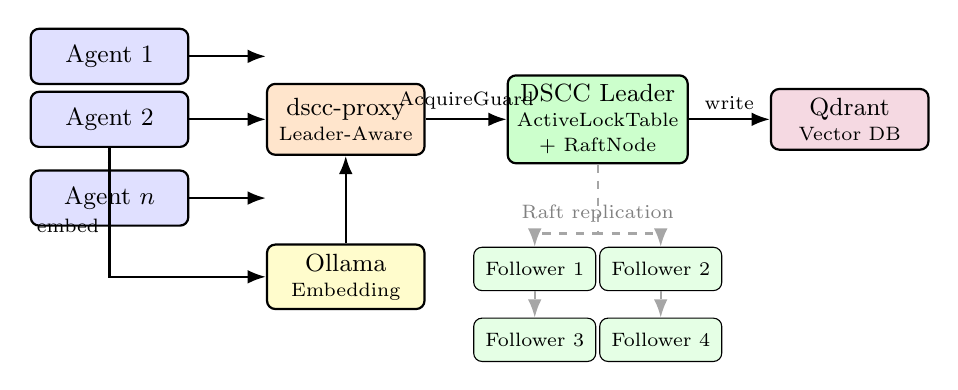
\begin{tikzpicture}[
      box/.style={draw, rounded corners=3pt, thick,
                  minimum height=0.70cm, minimum width=2.0cm,
                  font=\small, align=center},
      sbox/.style={draw, rounded corners=3pt,
                   minimum height=0.55cm, minimum width=1.55cm,
                   font=\scriptsize, align=center},
      arr/.style={-Latex, thick},
      darr/.style={-Latex, thick, dashed, gray!70}
    ]

    %% ---- fixed coordinate layout ----
    %% Agents column
    \node[box, fill=blue!12] at (0, 0.8)  (a1) {Agent 1};
    \node[box, fill=blue!12] at (0, 0.0)  (a2) {Agent 2};
    \node[font=\normalsize]  at (0,-0.45) (vd) {$\vdots$};
    \node[box, fill=blue!12] at (0,-1.0)  (an) {Agent $n$};

    %% Proxy
    \node[box, fill=orange!20, minimum height=0.90cm] at (3.0, 0.0) (proxy)
          {dscc-proxy\\[-2pt]{\scriptsize Leader-Aware}};

    %% Ollama (below proxy)
    \node[box, fill=yellow!20] at (3.0, -2.0) (ollama)
          {Ollama\\[-2pt]{\scriptsize Embedding}};

    %% Leader
    \node[box, fill=green!20, minimum height=1.10cm, minimum width=2.2cm]
          at (6.2, 0.0) (leader)
          {DSCC Leader\\[-2pt]{\scriptsize ActiveLockTable}\\[-2pt]{\scriptsize + RaftNode}};

    %% Qdrant
    \node[box, fill=purple!15] at (9.4, 0.0) (qdrant)
          {Qdrant\\[-2pt]{\scriptsize Vector DB}};

    %% Followers  (two rows, two columns, below leader)
    \node[sbox, fill=green!10] at (5.4, -1.9) (f1) {Follower 1};
    \node[sbox, fill=green!10] at (7.0, -1.9) (f2) {Follower 2};
    \node[sbox, fill=green!10] at (5.4, -2.8) (f3) {Follower 3};
    \node[sbox, fill=green!10] at (7.0, -2.8) (f4) {Follower 4};

    %% ---- edges ----

    %% agents → proxy (straight horizontal lines at each agent's height)
    \draw[arr] (a1.east) -- (proxy.west |- a1.east);
    \draw[arr] (a2.east) -- (proxy.west);
    \draw[arr] (an.east) -- (proxy.west |- an.east);

    %% agents → Ollama (agent 2 goes straight down then right)
    \draw[arr] (a2.south) -- (0,-2.0) node[left, font=\scriptsize, pos=0.6] {embed}
               -- (ollama.west);

    %% Ollama → proxy (straight up)
    \draw[arr] (ollama.north) -- (proxy.south);

    %% proxy → leader
    \draw[arr] (proxy.east) -- node[above, font=\scriptsize] {AcquireGuard}
               (leader.west);

    %% leader → Qdrant
    \draw[arr] (leader.east) -- node[above, font=\scriptsize] {write}
               (qdrant.west);

    %% leader → followers (Raft replication, dashed)
    \draw[darr] (leader.south) -- (6.2,-1.45) -- (5.4,-1.45) -- (f1.north);
    \draw[darr] (leader.south) -- (6.2,-1.45) -- (7.0,-1.45) -- (f2.north);
    \draw[darr] (f1.south) -- (f3.north);
    \draw[darr] (f2.south) -- (f4.north);

    %% Raft label
    \node[font=\scriptsize, gray] at (6.2, -1.20) {Raft replication};

  \end{tikzpicture}
  \caption{DSCC system architecture. Agents embed their payload via Ollama, then send
    \texttt{AcquireGuard} through the leader-aware proxy. The proxy forwards to the
    current Raft leader, which runs admission through the ActiveLockTable and replicates
    the decision to four followers (dashed) before returning. The committed write then
    proceeds to Qdrant.}
  \label{fig:arch}
\end{figure*}

Figure~\ref{fig:arch} shows the end-to-end architecture. The system has four runtime
layers: (1) the \textbf{embedding service} (Ollama), (2) the \textbf{leader-aware
proxy} (\texttt{dscc-proxy}), (3) the \textbf{five-node DSCC cluster}, and (4) the
\textbf{Qdrant vector database}. All inter-service communication uses gRPC.

\subsection{Embedding Service}

Before any lock operation, the agent's payload is vectorized by Ollama. The resulting
embedding vector is attached to the gRPC \texttt{AcquireRequest} alongside the similarity
threshold $\theta$. The lock table itself never interprets natural language; it only
compares floating-point vectors. This clean separation means the embedding model can be
swapped without changing the locking logic (see~\S\ref{sec:embedding}).

\subsection{Leader-Aware Proxy}
\label{sec:proxy}

\texttt{dscc-proxy} is a C++ gRPC server that shields clients from leader changes.
A background \texttt{LeaderPollLoop} issues \texttt{GetLeader} RPCs every 100\,ms to
maintain a cached view of the current leader address. Client-facing requests are forwarded
via \texttt{Forward\-With\-Leader\-Retry}: if the first attempt fails or returns a
``not leader'' error, the proxy refreshes its leader cache and retries, up to three
attempts with a 35-second per-attempt deadline. gRPC channels to DSCC nodes are lazily
created and cached; the proxy does not open a connection to a node until the first
request destined for it.

\subsection{DSCC Cluster}

Each of the five DSCC nodes runs an identical binary that wires together a
\texttt{RaftNode}, an \texttt{ActiveLockTable}, and a \texttt{Lock\-Service\-Impl} (the
gRPC service handler). Only the leader accepts \texttt{AcquireGuard} and
\texttt{ReleaseGuard} requests. Followers maintain a replica of the lock state through
Raft log application and are ready to become leader if the current leader fails.

The cluster is deployed on Docker Compose. Each node is allocated its own container, and
Qdrant runs in a sixth container. Container resource limits for CPU and memory are
configured per-node to emulate heterogeneous hardware.

%% =====================================================================
\section{Raft Consensus Layer}
\label{sec:raft}

\subsection{Configuration and Threading}

The Raft cluster has $N{=}5$ nodes, requiring a quorum of 3 and tolerating 2
simultaneous failures. Each node runs three background threads: a \texttt{HeartbeatLoop}
(75\,ms period) that sends \texttt{AppendEntries} RPCs to all peers; an
\texttt{ElectionTimerLoop} (10\,ms poll, 600--1000\,ms randomized deadline) that
triggers candidate campaigns; and an \texttt{ApplyLoop} that delivers committed log
entries to the \texttt{on\_commit\_} callback.

\subsection{Two-Phase Admission}
\label{sec:two-phase}

A single \texttt{AcquireGuard} call on the leader traverses three phases:

\begin{enumerate}
\item \textbf{Admission (Phase 1).} \texttt{wait\_for\_admission()} blocks on the
  ActiveLockTable until no active lock conflicts with the incoming embedding. On
  clearance, it inserts a \emph{pending} slot — a reservation that participates in
  conflict detection before Raft commits (see~\S\ref{sec:pending}).

\item \textbf{Consensus (Phase 2).} The leader calls \texttt{Propose(ACQUIRE)}, which
  appends the entry to the Raft log and waits for a quorum \texttt{AppendEntries}
  acknowledgement via \texttt{WaitUntilApplied}.

\item \textbf{Promotion.} The \texttt{on\_commit\_} callback fires on every node.
  On the leader, \texttt{apply\_acquire()} finds the pending entry and clears the
  \texttt{pending} flag, promoting it to a real lock. On followers, no pending slot
  exists, so \texttt{apply\_acquire()} inserts a fresh real lock directly.
\end{enumerate}

The agent is then free to execute its Qdrant write. After the write completes,
\texttt{ReleaseGuard} issues \texttt{Propose(RELEASE)} and the lock is removed from
the table on all nodes through the same apply callback path.

\subsection{Pending Lock Semantics}
\label{sec:pending}

The pending flag solves a race between the end of Phase 1 and the completion of
Phase 2. Without a reservation, a second agent could observe the lock table between
the moment the first agent clears the conflict check and the moment the Raft commit
makes its lock visible. The pending slot closes this window: it participates in
\texttt{find\_conflict\_locked} immediately after \texttt{wait\_for\_admission} returns,
before any Raft round-trip.

\subsection{Ghost Lock Prevention}
\label{sec:ghost}

If \texttt{Propose(ACQUIRE)} times out or the leader loses leadership during Phase 2,
the pending slot must be cleaned up. The leader calls \texttt{remove\_\-pending(agent\_id)},
which removes the pending entry and rebalances any waiters queued behind it — but only
if the entry is still pending. If the Raft commit had already promoted it, a compensating
\texttt{Propose(RELEASE)} is submitted instead (\emph{AppendLocalEntry} path). This
ensures that ghost locks — pending entries that were never promoted but also never
removed — cannot accumulate and block the system indefinitely.

\subsection{Sequential Vote Collection — A Known Limitation}
\label{sec:raft-limit}

Vote requests during leader election are currently issued sequentially rather than in
parallel, giving $O(N \times \text{rpc\_timeout})$ election time in the worst case.
On a healthy local Docker network this is acceptable, but on a high-latency WAN it would
significantly delay recovery. Additionally, the implementation lacks a \emph{pre-vote}
phase~\cite{raft}: a temporarily partitioned node can increment its term and disrupt the
cluster on reconnect. Both are identified as open limitations in~\S\ref{sec:limitations}.

%% =====================================================================
\section{The ActiveLockTable}
\label{sec:lock-table}

The ActiveLockTable is the central contribution of this paper. It is an in-memory
concurrent data structure that answers two questions for every incoming request:
\emph{``Does this request conflict with any active lock?''} and, if so,
\emph{``Who should this request wait behind, and in what position?''}

\subsection{Early Design and Its Failure Mode}

The initial implementation used the simplest possible representation: a flat
\texttt{vector<SemanticLock>} protected by a single mutex and a single global
\texttt{condition\_variable}:

\begin{lstlisting}[caption={Early single-CV design}]
class ActiveLockTable {
    std::vector<SemanticLock> active_;
    mutable std::mutex mu_;
    std::condition_variable cv_;  // shared by all waiters
};
\end{lstlisting}

When any lock was released, \texttt{cv\_.notify\_all()} woke \emph{every} blocked thread.
Each woken thread then re-evaluated the conflict predicate under the mutex. In the
thundering-herd test case (13 agents competing for a single semantic region), this caused
a burst of 12 simultaneous wakeups, 11 of which immediately went back to sleep after
re-discovering a conflict. Under contention, the mutex became a serialization point for
all woken threads, and the lock table throughput degraded nearly linearly with the number
of waiting agents.

Additionally, the flat vector required $O(n)$ scans for both conflict checks and lock
removal, and there was no concept of per-lock waiter ordering — a newly woken thread
could jump ahead of a thread that had been waiting longer, violating FIFO fairness.

\subsection{Current Data Model}

The production design replaces the vector and shared CV with two structural changes:

\begin{lstlisting}[caption={Current per-waiter CV design}]
struct WaitQueueEntry {
    std::string waiting_agent_id;
    std::vector<float> embedding;
    float theta;
    std::shared_ptr<std::condition_variable> cv;
    bool ready{false};
    bool granted{false};
    int queue_hops{0};
};

struct SemanticLock {
    std::string agent_id;
    std::vector<float> centroid;
    float threshold;
    bool pending;
    std::deque<std::shared_ptr<WaitQueueEntry>> waiters;
};

class ActiveLockTable {
    std::unordered_map<std::string, SemanticLock> active_;
    mutable std::mutex mu_;
    // No shared CV — each WaitQueueEntry has its own.
};
\end{lstlisting}

\noindent Key design choices:

\textbf{Per-lock FIFO deque.} Each \texttt{SemanticLock} owns a
\texttt{deque} of \texttt{Wait\-Queue\-Entry} objects, not a flat list of all blocked
threads. When a lock is released, only the waiters attached to that lock are processed.

\textbf{Per-waiter condition variable.} Every \texttt{Wait\-Queue\-Entry} has its own
\texttt{condition\_variable}. The rebalancer notifies only the CVs of threads it
decides to grant, not all threads. This eliminates the thundering herd entirely.

\textbf{Two wakeup reasons.} The \texttt{ready} flag gates the CV wait; \texttt{granted}
distinguishes a grant handoff (the rebalancer already inserted a pending slot and the
thread must not re-run the conflict check) from a spurious wakeup (the thread re-enters
the while loop).

\textbf{$O(1)$ lookup.} The \texttt{unordered\_map} keyed by \texttt{agent\_id} gives
constant-time lock insertion, removal, and promotion from pending to real.

\subsection{Conflict Detection: Strongest-Blocker Selection}
\label{sec:conflict}

\texttt{find\_conflict\_locked} scans all entries in \texttt{active\_} and computes
cosine similarity between the incoming embedding and each lock's centroid
(Equation~\ref{eq:conflict}). If multiple locks conflict, the waiter is attached to the
one with the \emph{highest} similarity — the strongest blocker:

\begin{lstlisting}[caption={Strongest-blocker selection}]
ConflictTrace best;
for (auto& [agent_id, entry] : active_) {
    float sim = cosine_similarity(embedding, entry.centroid);
    if (sim >= threshold &&
        (best.lock == nullptr || sim >= best.similarity)) {
        best.lock = &entry;
        best.similarity = sim;
    }
}
return best;
\end{lstlisting}

\noindent The rationale is that a waiter attached to its most semantically similar
blocker will experience the minimal number of requeue hops: when the strongest blocker
releases, the waiter is most likely to pass the re-evaluation. Attaching to a weaker
blocker that releases earlier would require the waiter to be requeued behind the stronger
one, adding a hop and additional latency.

\noindent\textbf{Threshold asymmetry.} The conflict check always uses the
\emph{incoming} request's $\theta$, not the active lock's. A conservative client with
low $\theta$ can therefore be blocked by an active lock that would not have considered
the new request a conflict at its own threshold.

\subsection{The Rebalancer: \texttt{rebalance\_\-waiters\_\-locked}}
\label{sec:rebalancer}

When a lock is released, its waiter deque is detached and passed to
\texttt{rebalance\_\-waiters\_\-locked}. The rebalancer processes waiters front-to-back
(FIFO order):

\begin{lstlisting}[caption={Rebalancer core loop}]
while (!waiters.empty()) {
    auto waiter = waiters.front();
    waiters.pop_front();

    ConflictTrace conflict =
        find_conflict_locked(waiter->embedding, waiter->theta);

    if (conflict.lock != nullptr) {
        // Still blocked — requeue behind new strongest blocker
        ++waiter->queue_hops;
        conflict.lock->waiters.push_back(waiter);
        continue;
    }

    // Granted — insert pending slot and notify after mu_ released
    insert_pending_locked(waiter->waiting_agent_id,
                          waiter->embedding, waiter->theta);
    waiter->granted = true;
    waiter->ready  = true;
    granted_waiters.push_back(std::move(waiter));
}
\end{lstlisting}

\noindent All mutations happen under \texttt{mu\_}. CV notifications fire \emph{after}
\texttt{mu\_} is released, preventing a waking thread from contending with ongoing
rebalancing.

\subsection{Cascading Grant Effect}
\label{sec:cascade}

The most subtle behavior arises when multiple waiters can be granted in a single
rebalance pass. Consider: active locks $X$ (agent A) and $Y$ (agent B), with
$X$'s waiters $[W_1, W_2]$. Agent A releases $X$. The rebalancer processes the detached
queue $[W_1, W_2]$:

\begin{enumerate}
\item $W_1$ is evaluated against $\{Y\}$. No conflict — $W_1$ is granted and inserted
  into \texttt{active\_} as pending. Now \texttt{active\_} $= \{Y, W_1\}$.
\item $W_2$ is evaluated against $\{Y, W_1\}$. If $W_2$ conflicts with $W_1$,
  $W_2$ is requeued behind $W_1$, with \texttt{queue\_hops} incremented.
  If $W_2$ does not conflict with either, $W_2$ is also granted.
\end{enumerate}

\noindent The key insight is that granting $W_1$ can \emph{block} $W_2$ in the same
rebalance pass. Because the rebalancer processes front-to-back, earlier waiters get
priority — FIFO fairness is preserved within the conflict group. The
\texttt{queue\_hops} counter tracks how many times a waiter has been bounced across
lock queues; Figure~\ref{fig:timeline-cascade} shows this effect in the
Queue-Hopping benchmark case.

\subsection{Notification Safety}

After all rebalancing completes, \texttt{mu\_} is released and each granted waiter's
\texttt{cv->notify\_all()} is called. The waking thread finds \texttt{granted} set to \texttt{true},
skips the conflict re-check, and proceeds directly to \texttt{Propose(ACQUIRE)}. The
\texttt{Wait\-Queue\-Entry} shared pointer is kept alive by both the sleeping thread and
the granted-waiters list; the rebalancer's copy is dropped after notification.

%% =====================================================================
\section{Embedding Model as Conflict Predicate}
\label{sec:embedding}

\subsection{Why Model Choice Is Architectural}

The ActiveLockTable receives only floating-point vectors and a scalar threshold; it
contains no NLP logic. Therefore, the embedding model controls the \emph{geometry of the
lock space}: which payloads are considered conflicting, which can run in parallel, and
how the threshold should be interpreted. Two agents writing paraphrases of the same
intent will block each other only if the model places their embeddings above $\theta$. If
the model fails to cluster paraphrases tightly, the lock manager faithfully allows them
to run concurrently — producing a semantic race condition that no amount of consensus
correctness can fix.

We evaluated three models (Table~\ref{tab:models}) across three threshold values
($\theta \in \{0.55, 0.75, 0.95\}$) and 13 benchmark scenarios.

\begin{table}[t]
  \centering
  \caption{Evaluated embedding models}
  \label{tab:models}
  \begin{tabular}{lccc}
    \toprule
    Model & Dims & Emb. p50 & Emb. p99 \\
    \midrule
    \texttt{all-minilm:latest}       & 384  & 10\,ms   & 324\,ms  \\
    \texttt{bge-m3:latest}           & 1024 & 111\,ms  & 1774\,ms \\
    \texttt{qwen3-embedding:0.6b}    & 1024 & 133\,ms  & 1517\,ms \\
    \bottomrule
  \end{tabular}
\end{table}

\subsection{Paraphrase Gauntlet Results}

The Paraphrase Gauntlet (Case 11) presents 12 pairs of semantically equivalent sentences
drawn from distinct domains — sustainability design, legal reasoning, financial analysis —
to test whether the system correctly serializes each pair. Table~\ref{tab:gauntlet} shows
the serialization score and violation count at $\theta = 0.75$.

\begin{table}[t]
  \centering
  \caption{Paraphrase Gauntlet at $\theta = 0.75$}
  \label{tab:gauntlet}
  \begin{tabular}{lcc}
    \toprule
    Model & Serialization Score & Violations \\
    \midrule
    \texttt{all-minilm}   & 0.500 & 6 \\
    \texttt{bge-m3}        & 0.750 & 3 \\
    \texttt{qwen3}         & \textbf{1.000} & \textbf{0} \\
    \bottomrule
  \end{tabular}
\end{table}

\noindent Only \texttt{qwen3-embedding:0.6b} at $\theta{=}0.75$ achieves a perfect
serialization score.

\begin{figure}[htbp]
  \centering
  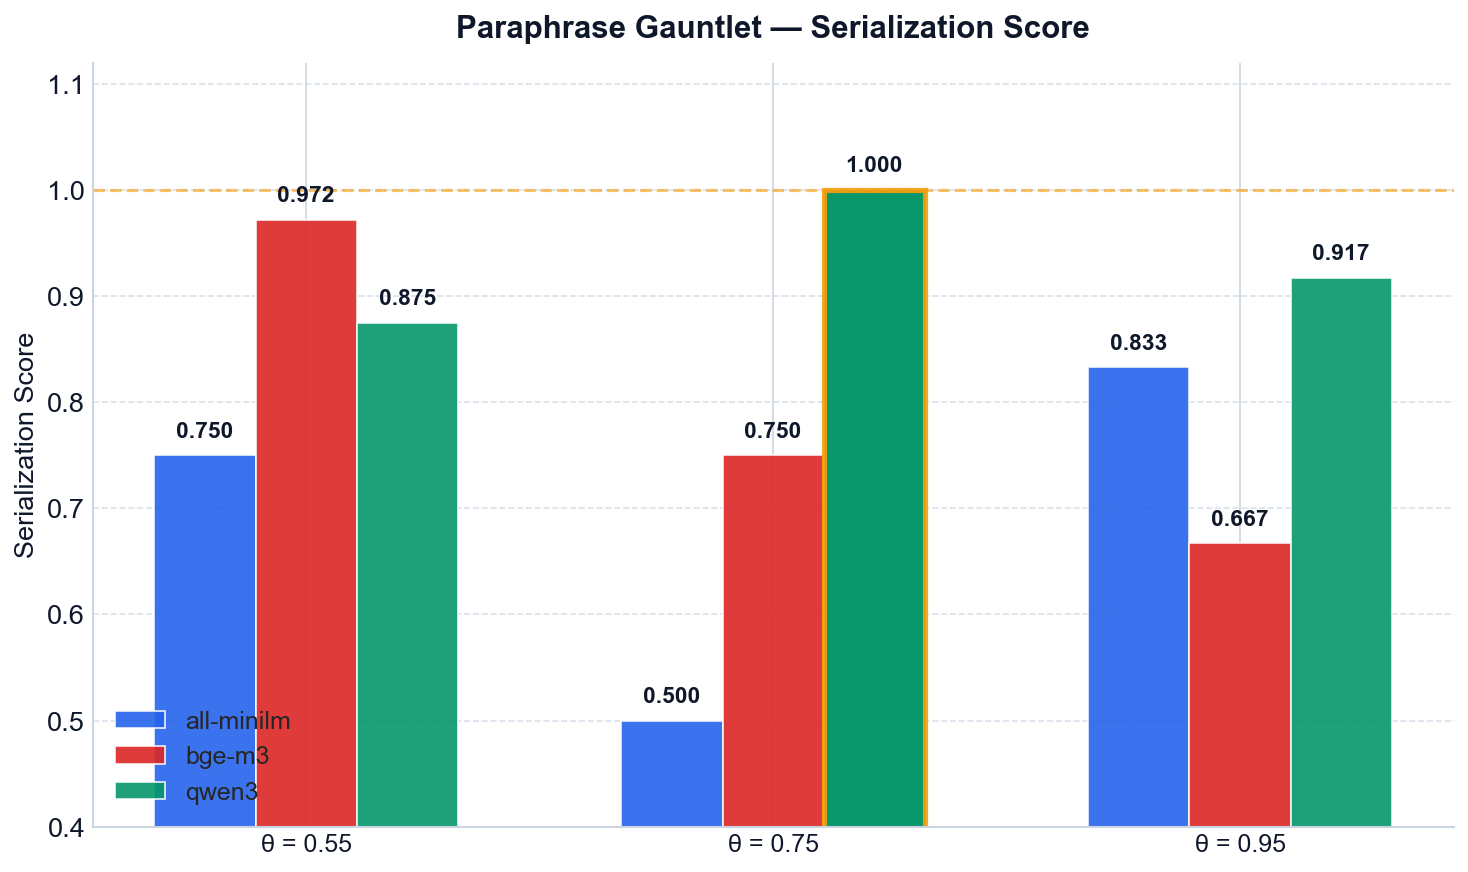
\includegraphics[width=\columnwidth,height=5.5cm,keepaspectratio]{scripts/plots/result_slides/01_paraphrase_gauntlet_ser_score.png}
  \caption{Serialization scores across all three models and three threshold values on the
    Paraphrase Gauntlet. \texttt{qwen3} at $\theta{=}0.75$ is the only combination
    achieving a score of 1.000.}
  \label{fig:serscores}
\end{figure}

\begin{figure}[htbp]
  \centering
  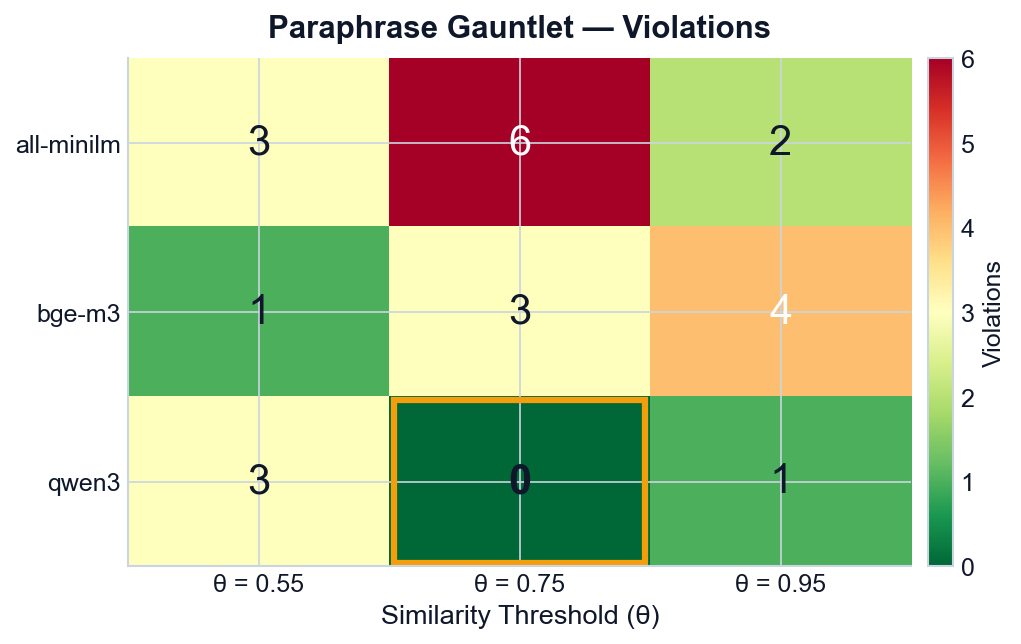
\includegraphics[width=\columnwidth,height=5.5cm,keepaspectratio]{scripts/plots/result_slides/02_violation_heatmap.png}
  \caption{Violation heatmap across models and threshold values. Darker cells indicate
    more paraphrase race conditions observed. \texttt{all-minilm} produces the most
    violations at every tested threshold.}
  \label{fig:vheatmap}
\end{figure}

Figure~\ref{fig:serscores} shows the full serialization score surface. The
non-monotonic behavior of \texttt{all-minilm} across thresholds illustrates why
lowering $\theta$ does not compensate for a weak paraphrase model: a lower threshold
increases blocking, but the wrong operations are being blocked. Figure~\ref{fig:vheatmap}
confirms that \texttt{all-minilm} accumulates the most violations at every threshold.

\subsection{Precision, Recall, and the False-Negative Risk}

\begin{figure}[htbp]
  \centering
  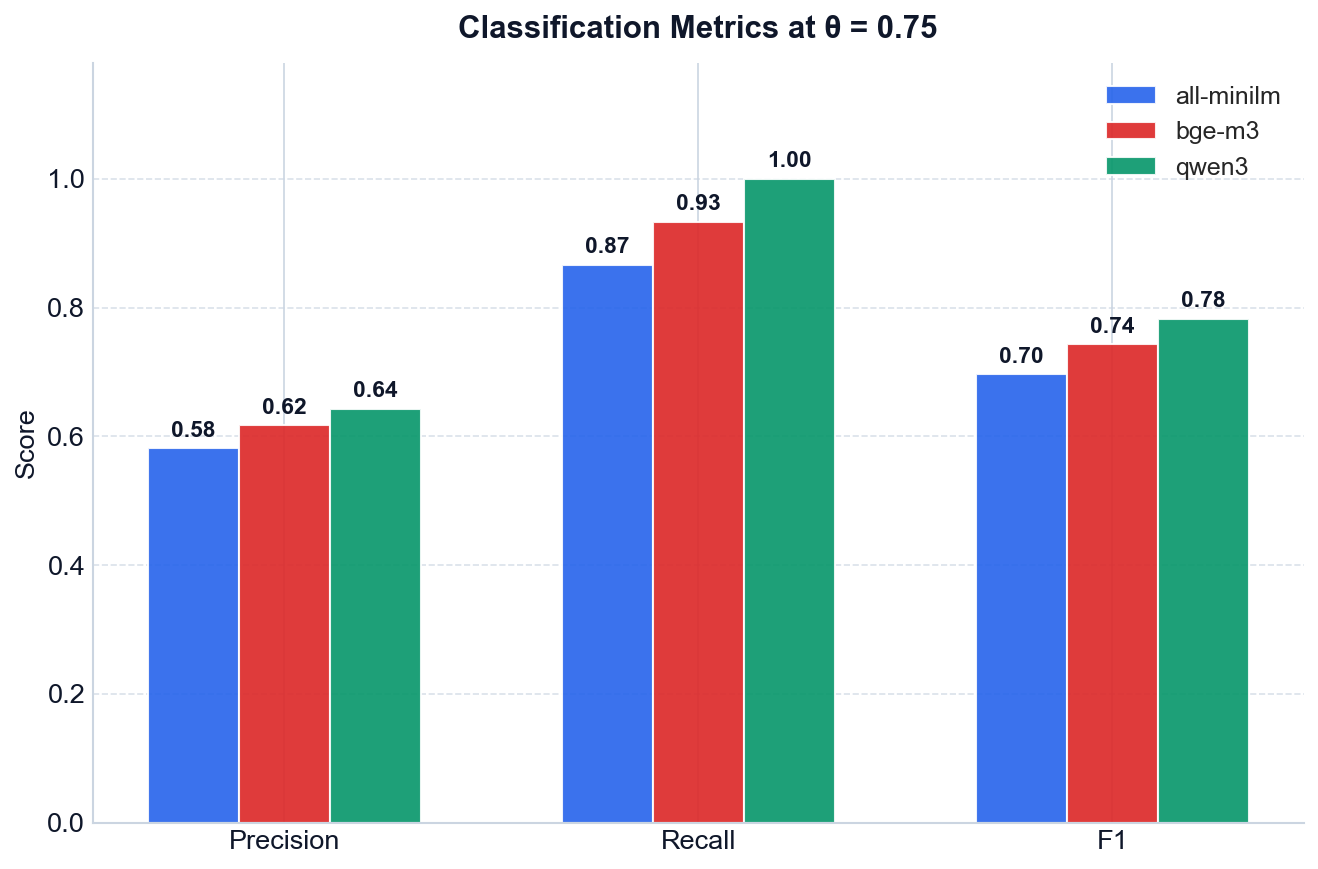
\includegraphics[width=\columnwidth,height=6cm,keepaspectratio]{scripts/plots/result_slides/04_precision_recall_f1.png}
  \caption{Precision, Recall, and F1 across models and threshold values. Higher recall
    is critical; a false negative is a semantic race condition.}
  \label{fig:prf}
\end{figure}

We frame conflict detection as binary classification: a true positive is a conflicting
pair that was serialized; a false negative is a conflicting pair that was allowed to race.
Figure~\ref{fig:prf} shows precision, recall, and F1. A false negative is strictly more
dangerous than a false positive (excessive blocking): missed paraphrase conflicts corrupt
the shared memory store, while over-blocking merely reduces throughput. The evaluation
therefore prioritizes recall over precision.

\subsection{Confusion Matrices at $\theta = 0.75$}

\begin{figure*}[t]
  \centering
  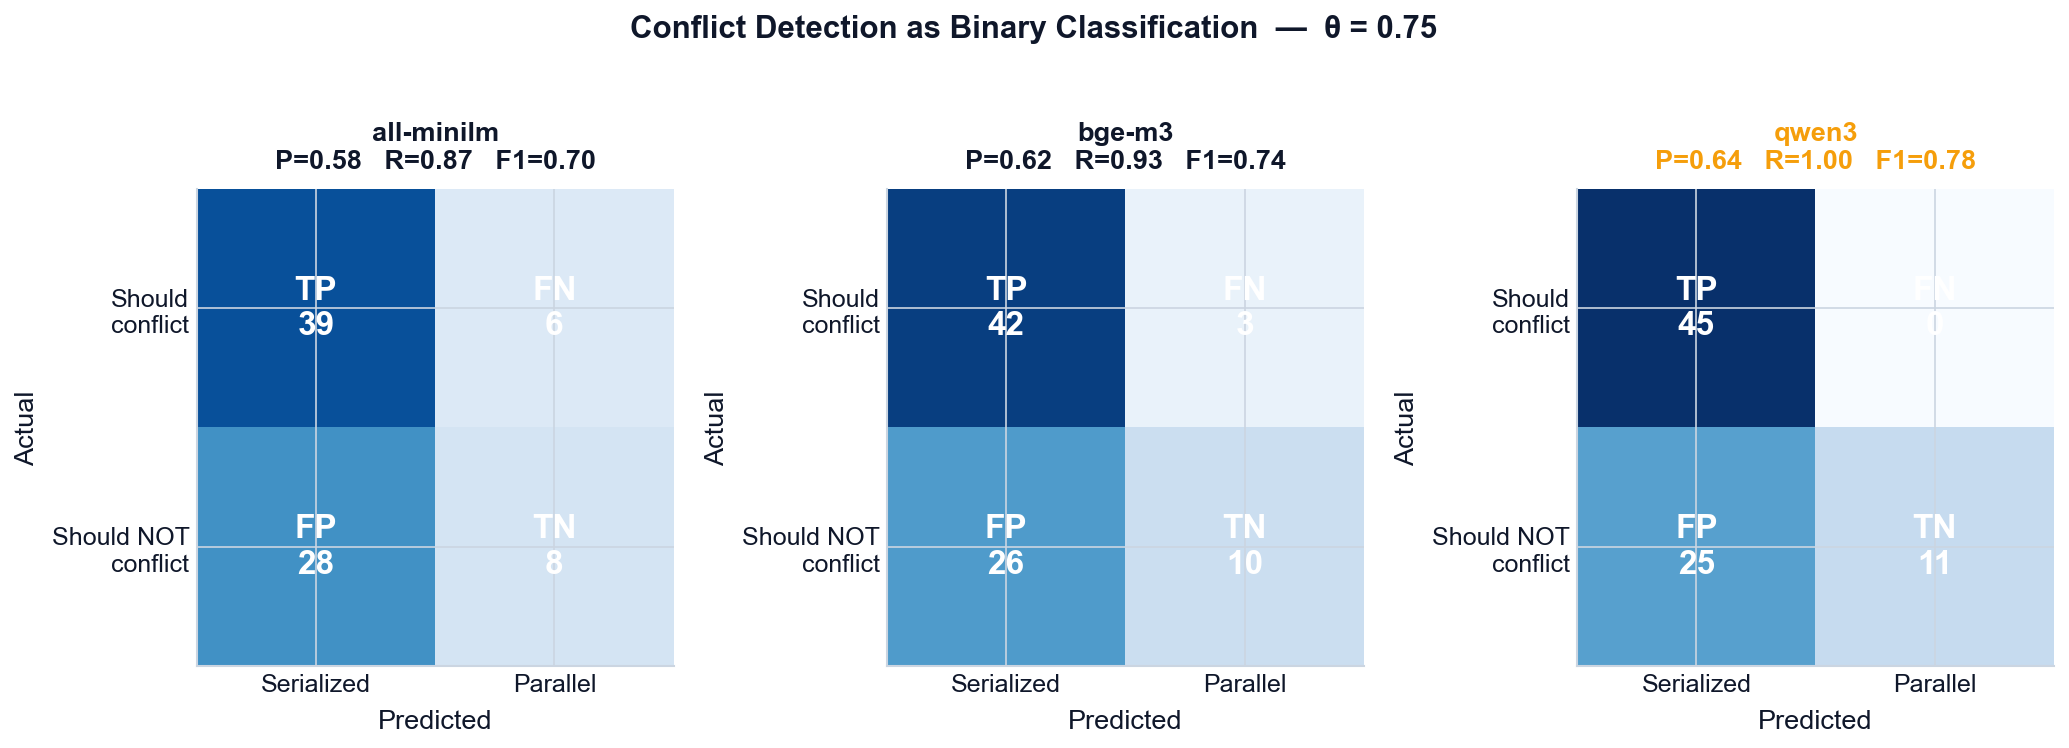
\includegraphics[width=\linewidth]{scripts/plots/result_slides/03_confusion_matrices_theta075.png}
  \caption{Per-model confusion matrices at $\theta{=}0.75$. Each cell counts (conflict
    pair, outcome) combinations. \texttt{qwen3} has zero false negatives; \texttt{all-minilm}
    has 6 false negatives corresponding to the 6 paraphrase violations.}
  \label{fig:confusion}
\end{figure*}

Figure~\ref{fig:confusion} provides per-model confusion matrices at $\theta{=}0.75$.
The matrices confirm that \texttt{qwen3}'s advantage comes from recall: it produces zero
false negatives while maintaining comparable precision to the other models at this
threshold.

\subsection{Threshold Sensitivity}

Threshold calibration is model-specific. At $\theta{=}0.55$, both \texttt{bge-m3} and
\texttt{qwen3} exhibit severe cross-domain false-positive blocking in Case 12 (Cross-Domain
Flood), with distinct parallelism collapsing to 0.000 and operation P95 exceeding
5500\,ms. At $\theta{=}0.95$, paraphrase recall degrades for all models as pairs drift
below the threshold. The calibrated operating point — \texttt{qwen3} at $\theta{=}0.75$
— sits in the stable region: paraphrases serialize, unrelated domains proceed in parallel.

\subsection{Embedding Overhead}

\begin{figure}[htbp]
  \centering
  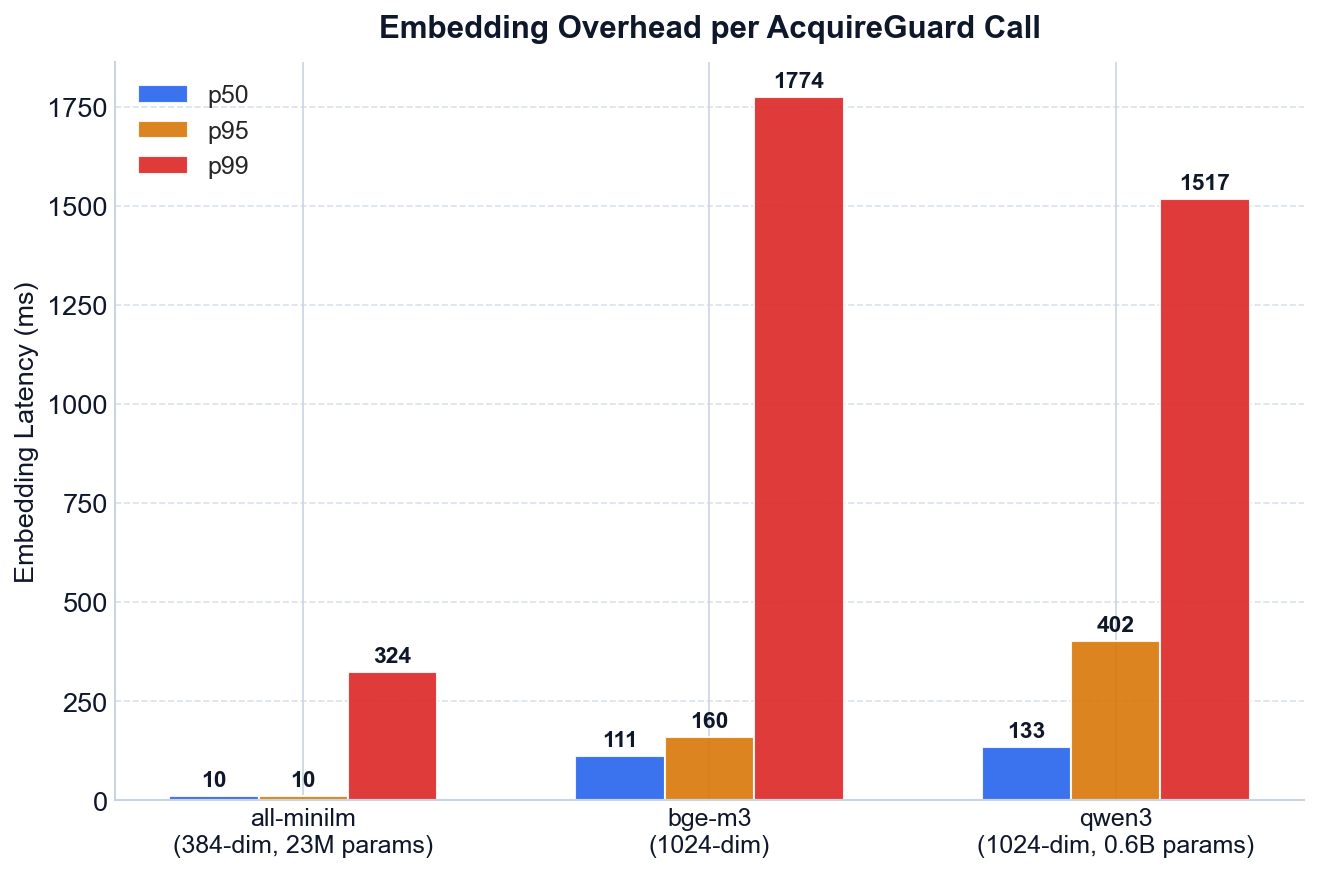
\includegraphics[width=\columnwidth,height=5.5cm,keepaspectratio]{scripts/plots/result_slides/06_embedding_overhead.png}
  \caption{Embedding latency distribution for the three models. \texttt{all-minilm}
    is fastest (p50 $\approx$ 10\,ms) but sacrifices semantic precision.
    \texttt{qwen3} has a p50 of 133\,ms, which is bounded and acceptable given
    that the Qdrant write and lock wait dominate end-to-end latency in contended
    scenarios.}
  \label{fig:emboverhead}
\end{figure}

Figure~\ref{fig:emboverhead} shows the embedding latency distribution. The p50 overhead
of 133\,ms for \texttt{qwen3} is bounded and predictable under steady load. In contended
scenarios the lock wait component dominates end-to-end latency by a wide margin; the
embedding overhead is a fixed per-request cost that does not scale with queue depth.

%% =====================================================================
\section{Evaluation}
\label{sec:eval}

\subsection{Benchmark Suite}
\label{sec:benchmark-suite}

The benchmark suite comprises 13 curated scenarios (C1--C13), each targeting a specific
correctness or performance property of the lock system. Scenarios are run in three
modes: \emph{single} (one model, one $\theta$), \emph{matrix} (three models $\times$
three $\theta$ values $\times$ 13 cases = 117 runs), and \emph{soak} (sustained load for
several minutes). Table~\ref{tab:cases} describes the 13 cases.

\begin{table}[t]
  \centering
  \caption{Benchmark scenario catalog}
  \label{tab:cases}
  \scriptsize
  \begin{tabular}{@{}clp{3.5cm}@{}}
    \toprule
    Case & Name & Purpose \\
    \midrule
    C1  & The Thundering Herd           & 13 agents, one semantic region; tests per-waiter CV design \\
    C2  & Semantic Interleaving         & Alternating related/unrelated writes; tests parallelism \\
    C3  & Read Starvation Trap          & Reader-writer priority under write pressure \\
    C4  & Permissive Sieve              & Low-$\theta$ blocking; tests false-positive rate \\
    C5  & Strict Sieve                  & High-$\theta$ blocking; tests false-negative rate \\
    C6  & Ghost Client                  & Proxy reconnect after leader change; tests ghost lock prevention \\
    C7  & Almost Collision              & Near-threshold pairs; boundary precision test \\
    C8  & Queue Hopping                 & Multiple conflict groups; tests queue\_hops counter \\
    C9  & Mixed Stagger                 & Time-staggered arrivals; tests fairness \\
    C10 & 100-Read Stampede             & Bulk reads with concurrent writes; throughput stress \\
    C11 & Paraphrase Gauntlet           & 12 paraphrase pairs; primary correctness test \\
    C12 & Cross-Domain Flood            & Unrelated domains; tests false-positive parallelism \\
    C13 & Write Pressure Ratchet        & Increasing write rate; latency under escalating load \\
    \bottomrule
  \end{tabular}
\end{table}

All runs execute inside Docker Compose on a single host. Each DSCC node runs in its own
container with CPU and memory limits. The benchmark runner (\texttt{benchmark\_runner.cpp})
orchestrates agent threads, collects per-operation timing, and writes JSON result files
consumed by the plotting pipeline.

\subsection{Agent Wait Time and Latency Decomposition}

\begin{figure}[htbp]
  \centering
  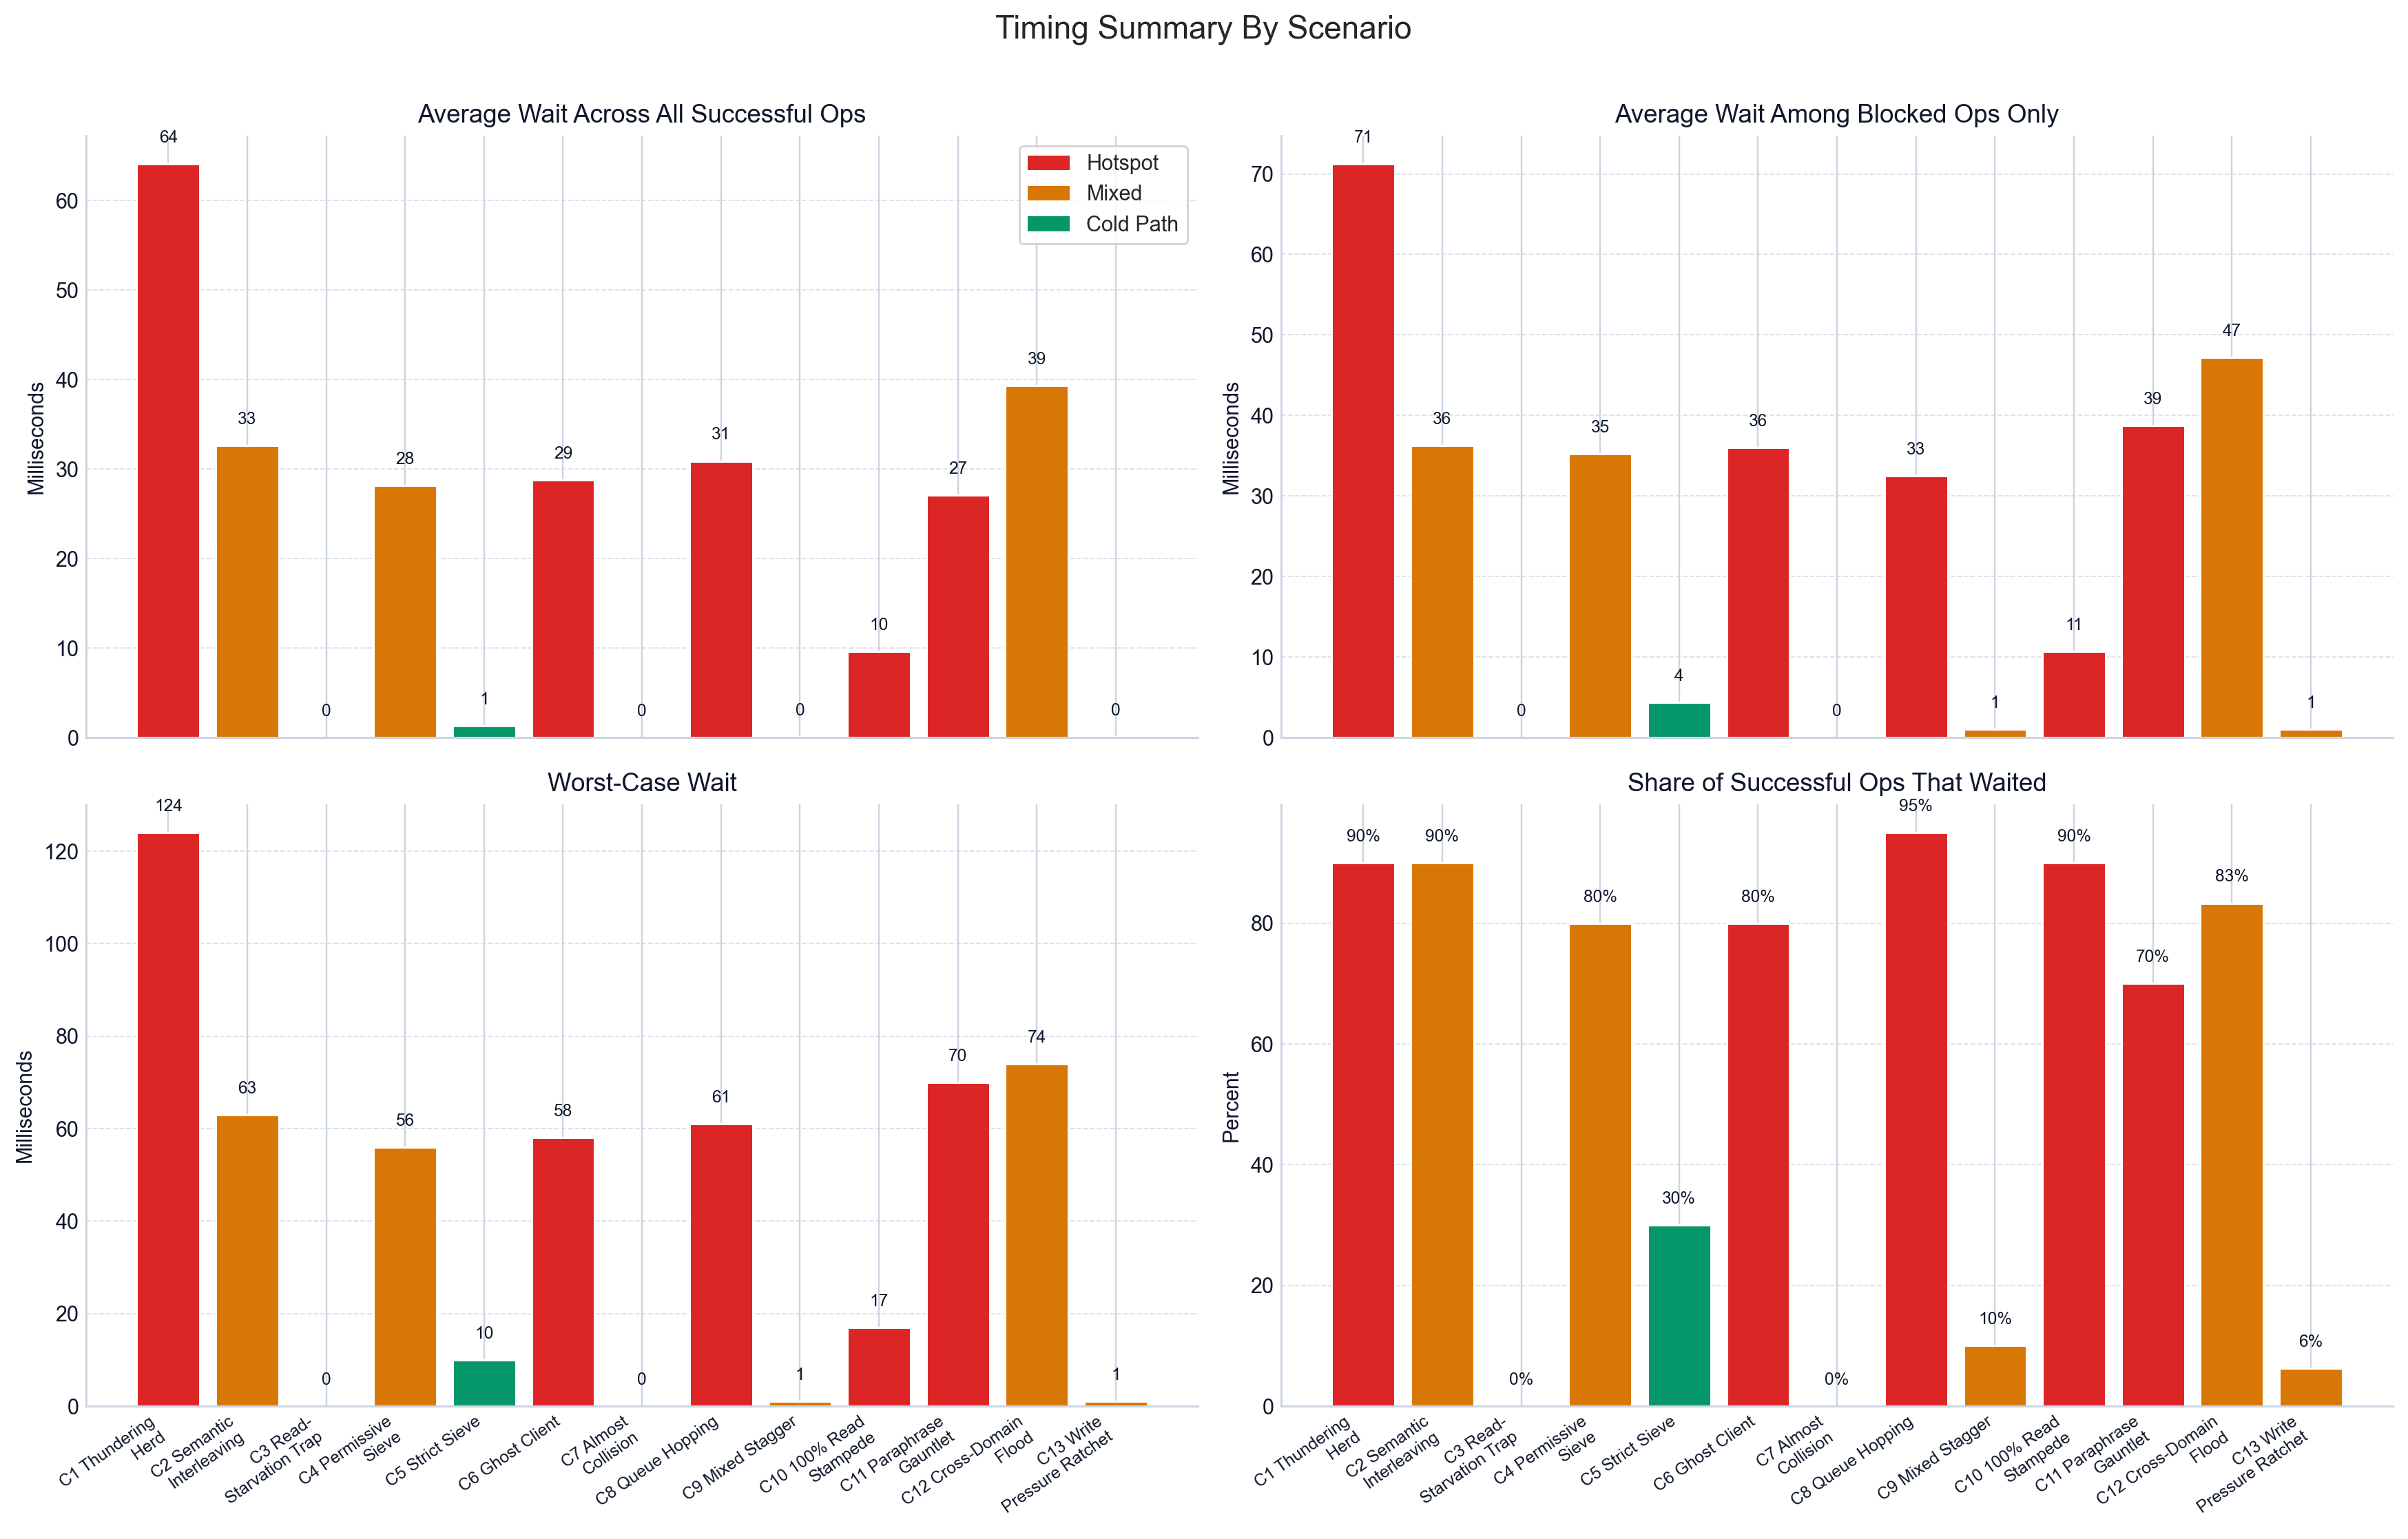
\includegraphics[width=\columnwidth,height=5.8cm,keepaspectratio]{scripts/plots/benchmark_run_1777321841/timing_01_wait_time_summary.png}
  \caption{Agent wait time summary across all 13 benchmark cases. C1 (Thundering Herd)
    and C11 (Paraphrase Gauntlet) show the highest median wait times.}
  \label{fig:waitsum}
\end{figure}

\begin{figure*}[t]
  \centering
  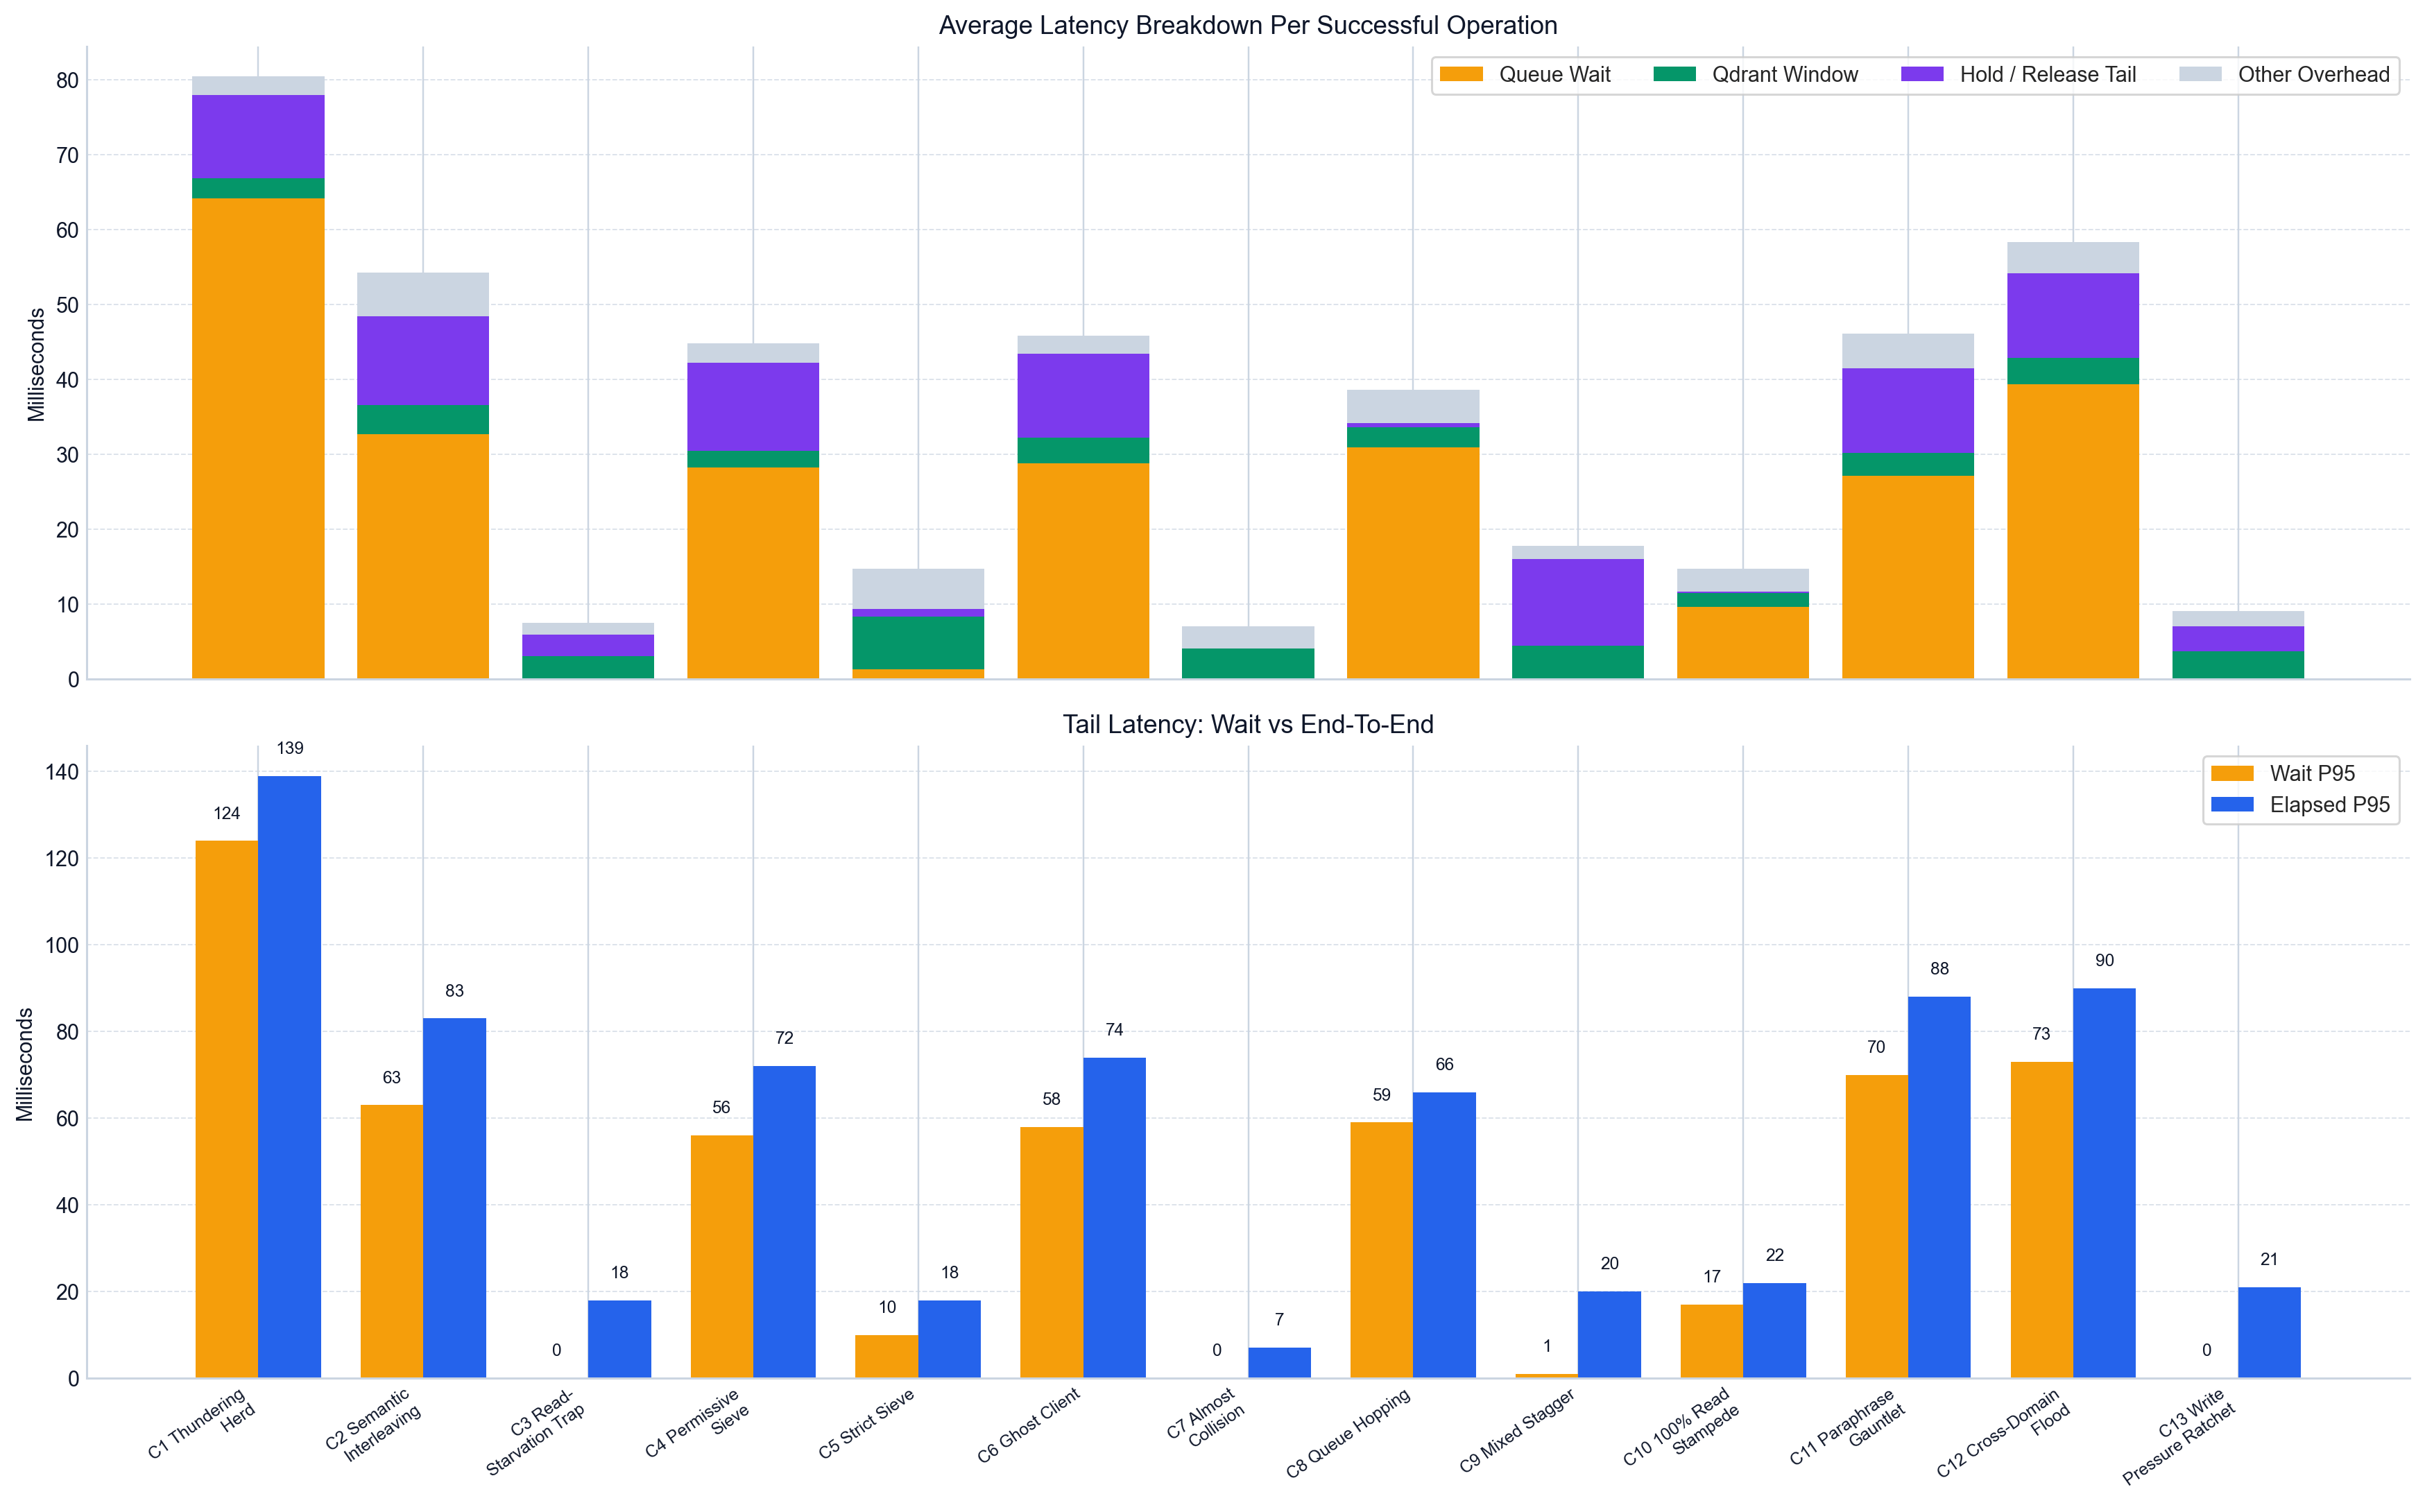
\includegraphics[width=\linewidth]{scripts/plots/benchmark_run_1777321841/timing_02_latency_component_breakdown.png}
  \caption{End-to-end latency broken down into four components: Queue Wait, Qdrant Write
    Window, Hold/Release Tail, and Other. In high-contention cases, Queue Wait dominates.
    Qdrant Write Window remains stable across cases, confirming that the vector store
    itself is not a bottleneck.}
  \label{fig:latcomp}
\end{figure*}

Figure~\ref{fig:waitsum} shows agent wait time across the 13 cases. Cases C1 and C11
exhibit the highest wait times, correctly reflecting deep queues in high-contention
semantic regions. Figure~\ref{fig:latcomp} decomposes end-to-end latency into four
components. Queue Wait dominates in contended cases; the Qdrant Write Window is stable
across all cases, confirming that the vector database is not a bottleneck.

\subsection{Case Studies: Thundering Herd and Queue Hopping}

\begin{figure}[htbp]
  \centering
  \begin{subfigure}[b]{\columnwidth}
    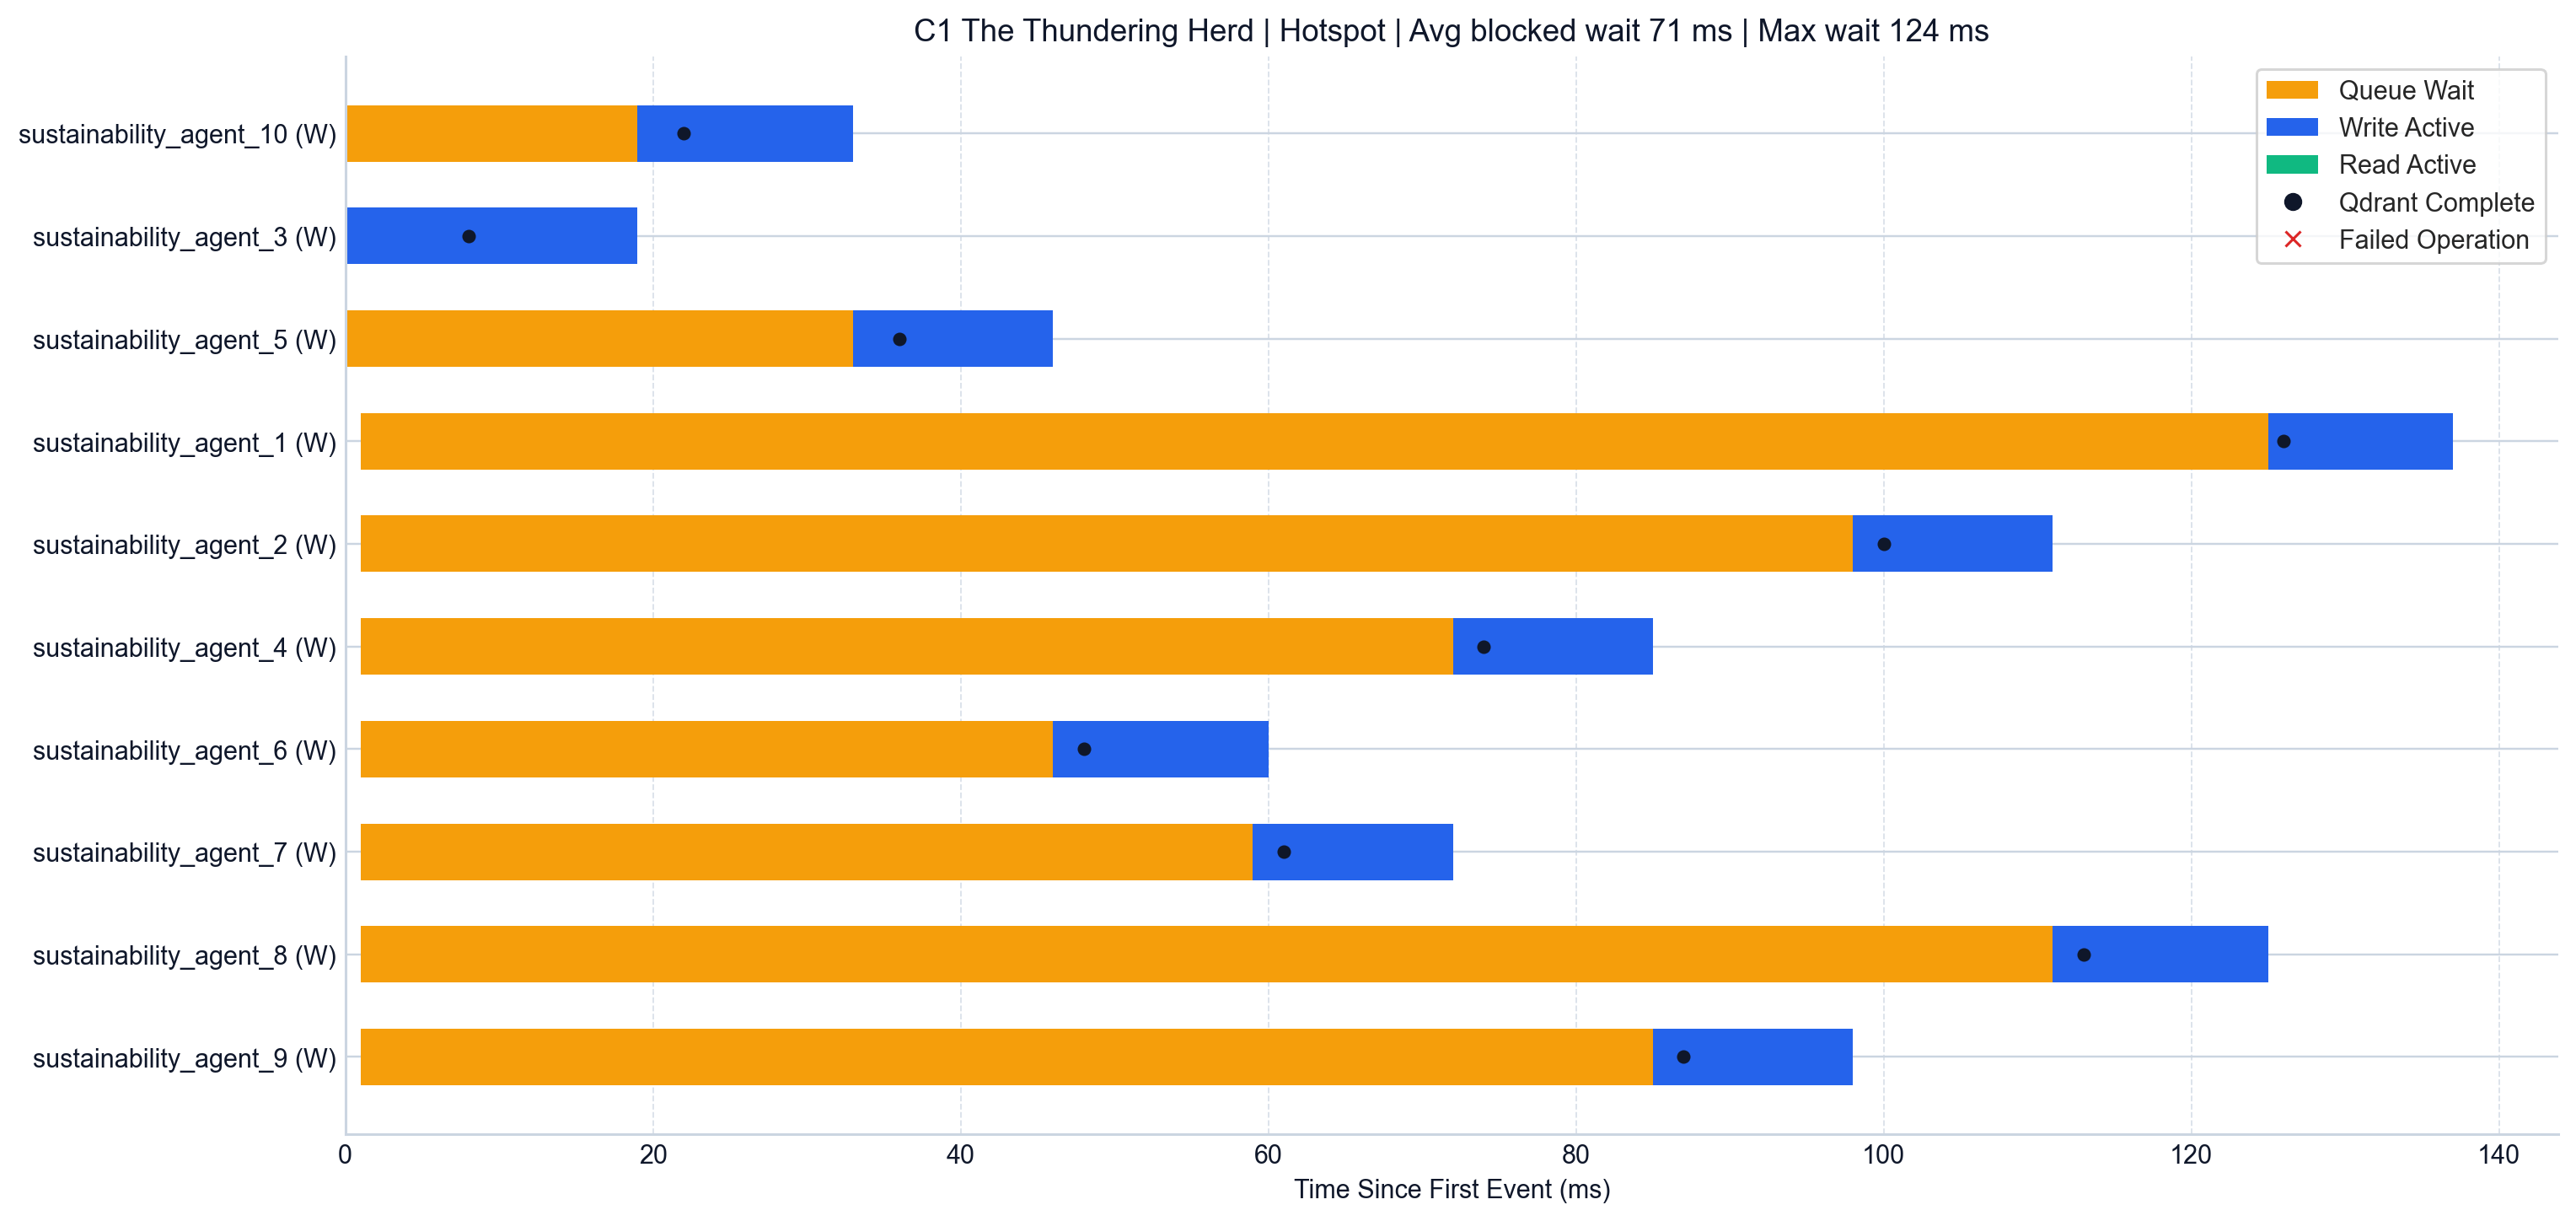
\includegraphics[width=\columnwidth,height=4.2cm,keepaspectratio]{scripts/plots/benchmark_run_1777321841/timing_timelines/timing_timeline_case_01_the_thundering_herd.png}
    \caption{C1: Thundering Herd — 13 agents serialized in FIFO order.}
    \label{fig:timeline-herd}
  \end{subfigure}
  \vspace{0.2em}
  \begin{subfigure}[b]{\columnwidth}
    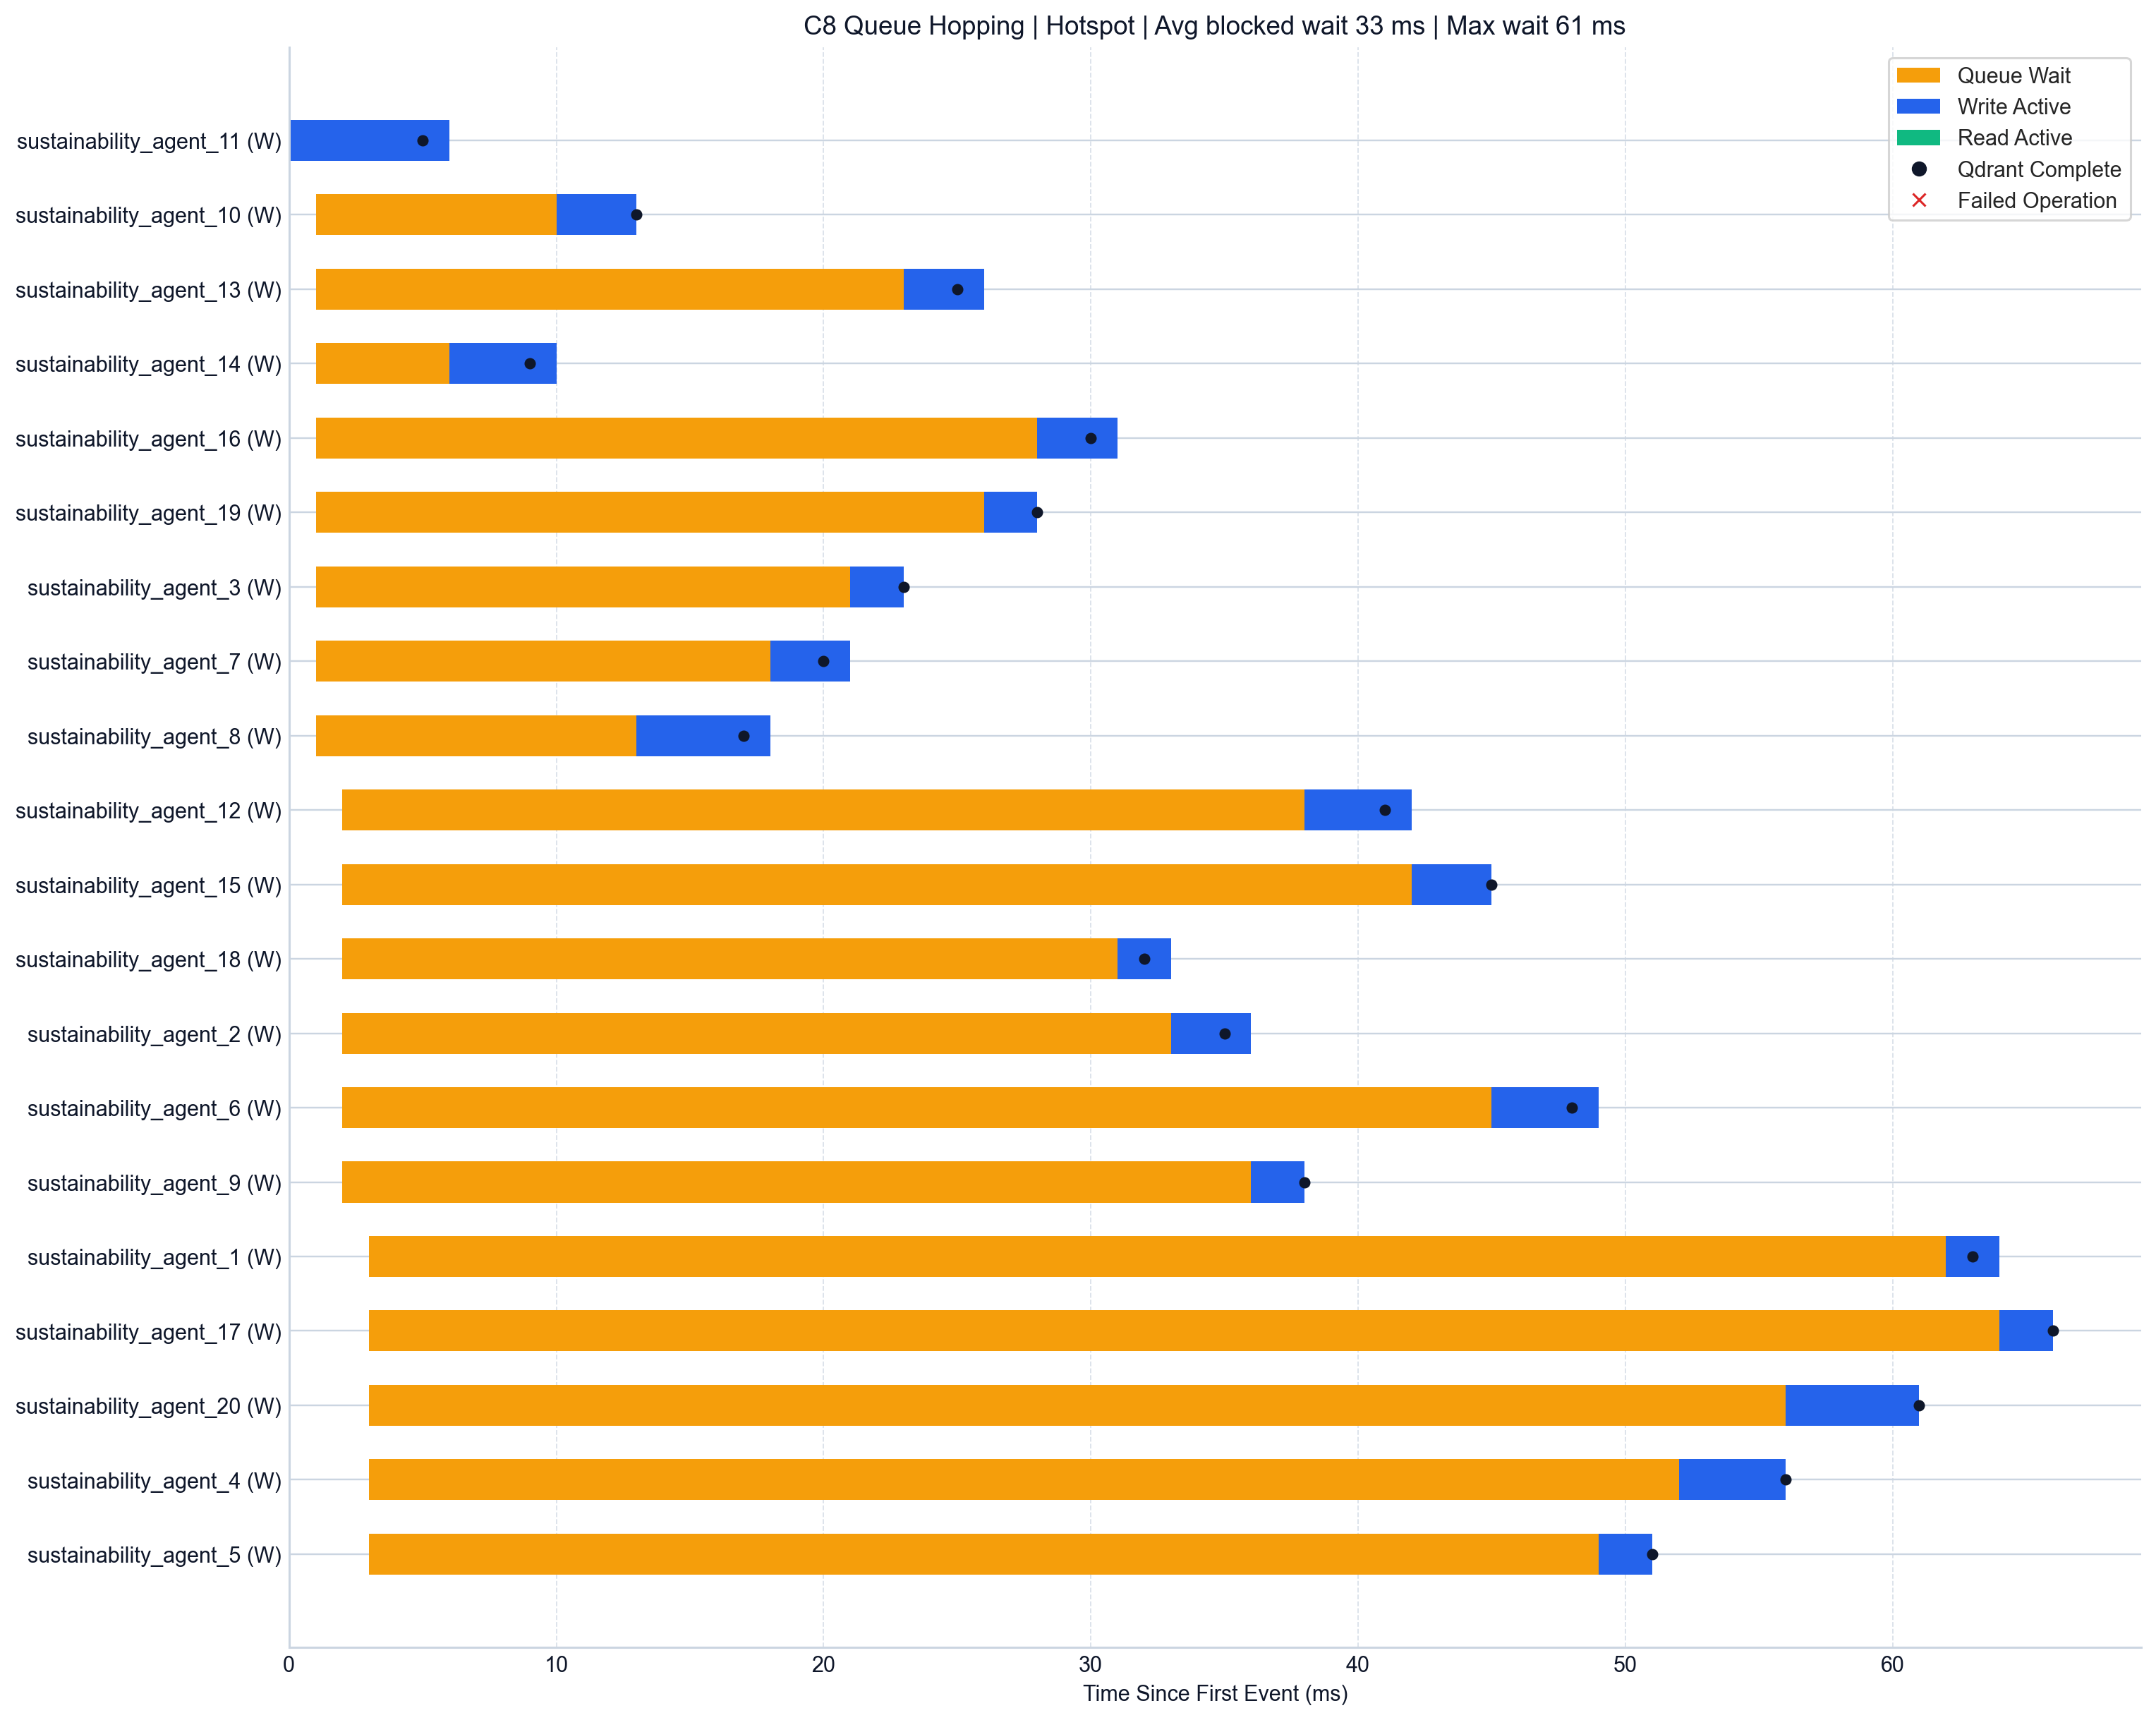
\includegraphics[width=\columnwidth,height=4.2cm,keepaspectratio]{scripts/plots/benchmark_run_1777321841/timing_timelines/timing_timeline_case_08_queue_hopping.png}
    \caption{C8: Queue Hopping — \texttt{queue\_hops} increments on each migration.}
    \label{fig:timeline-cascade}
  \end{subfigure}
  \caption{Agent-level timing timelines for selected benchmark cases.}
  \label{fig:timelines}
\end{figure}

Figure~\ref{fig:timelines} shows agent-level timelines for C1 and C8. In C1, all 13
agents arrive nearly simultaneously. Under the early single-CV design, all 12 waiting
threads would have been woken by the first release — a thundering herd. Under the current
per-waiter CV design, only the front-of-queue agent is woken, and the cascade proceeds
one agent at a time in FIFO order. In C8, agents migrate between conflict groups as
earlier waiters are granted and new pending slots appear; the timeline shows the
\texttt{queue\_hops} counter incrementing with each migration.

\subsection{Matrix Results: Latency, Fairness, and Blocked Rate}

\begin{figure}[htbp]
  \centering
  \begin{subfigure}[b]{0.48\columnwidth}
    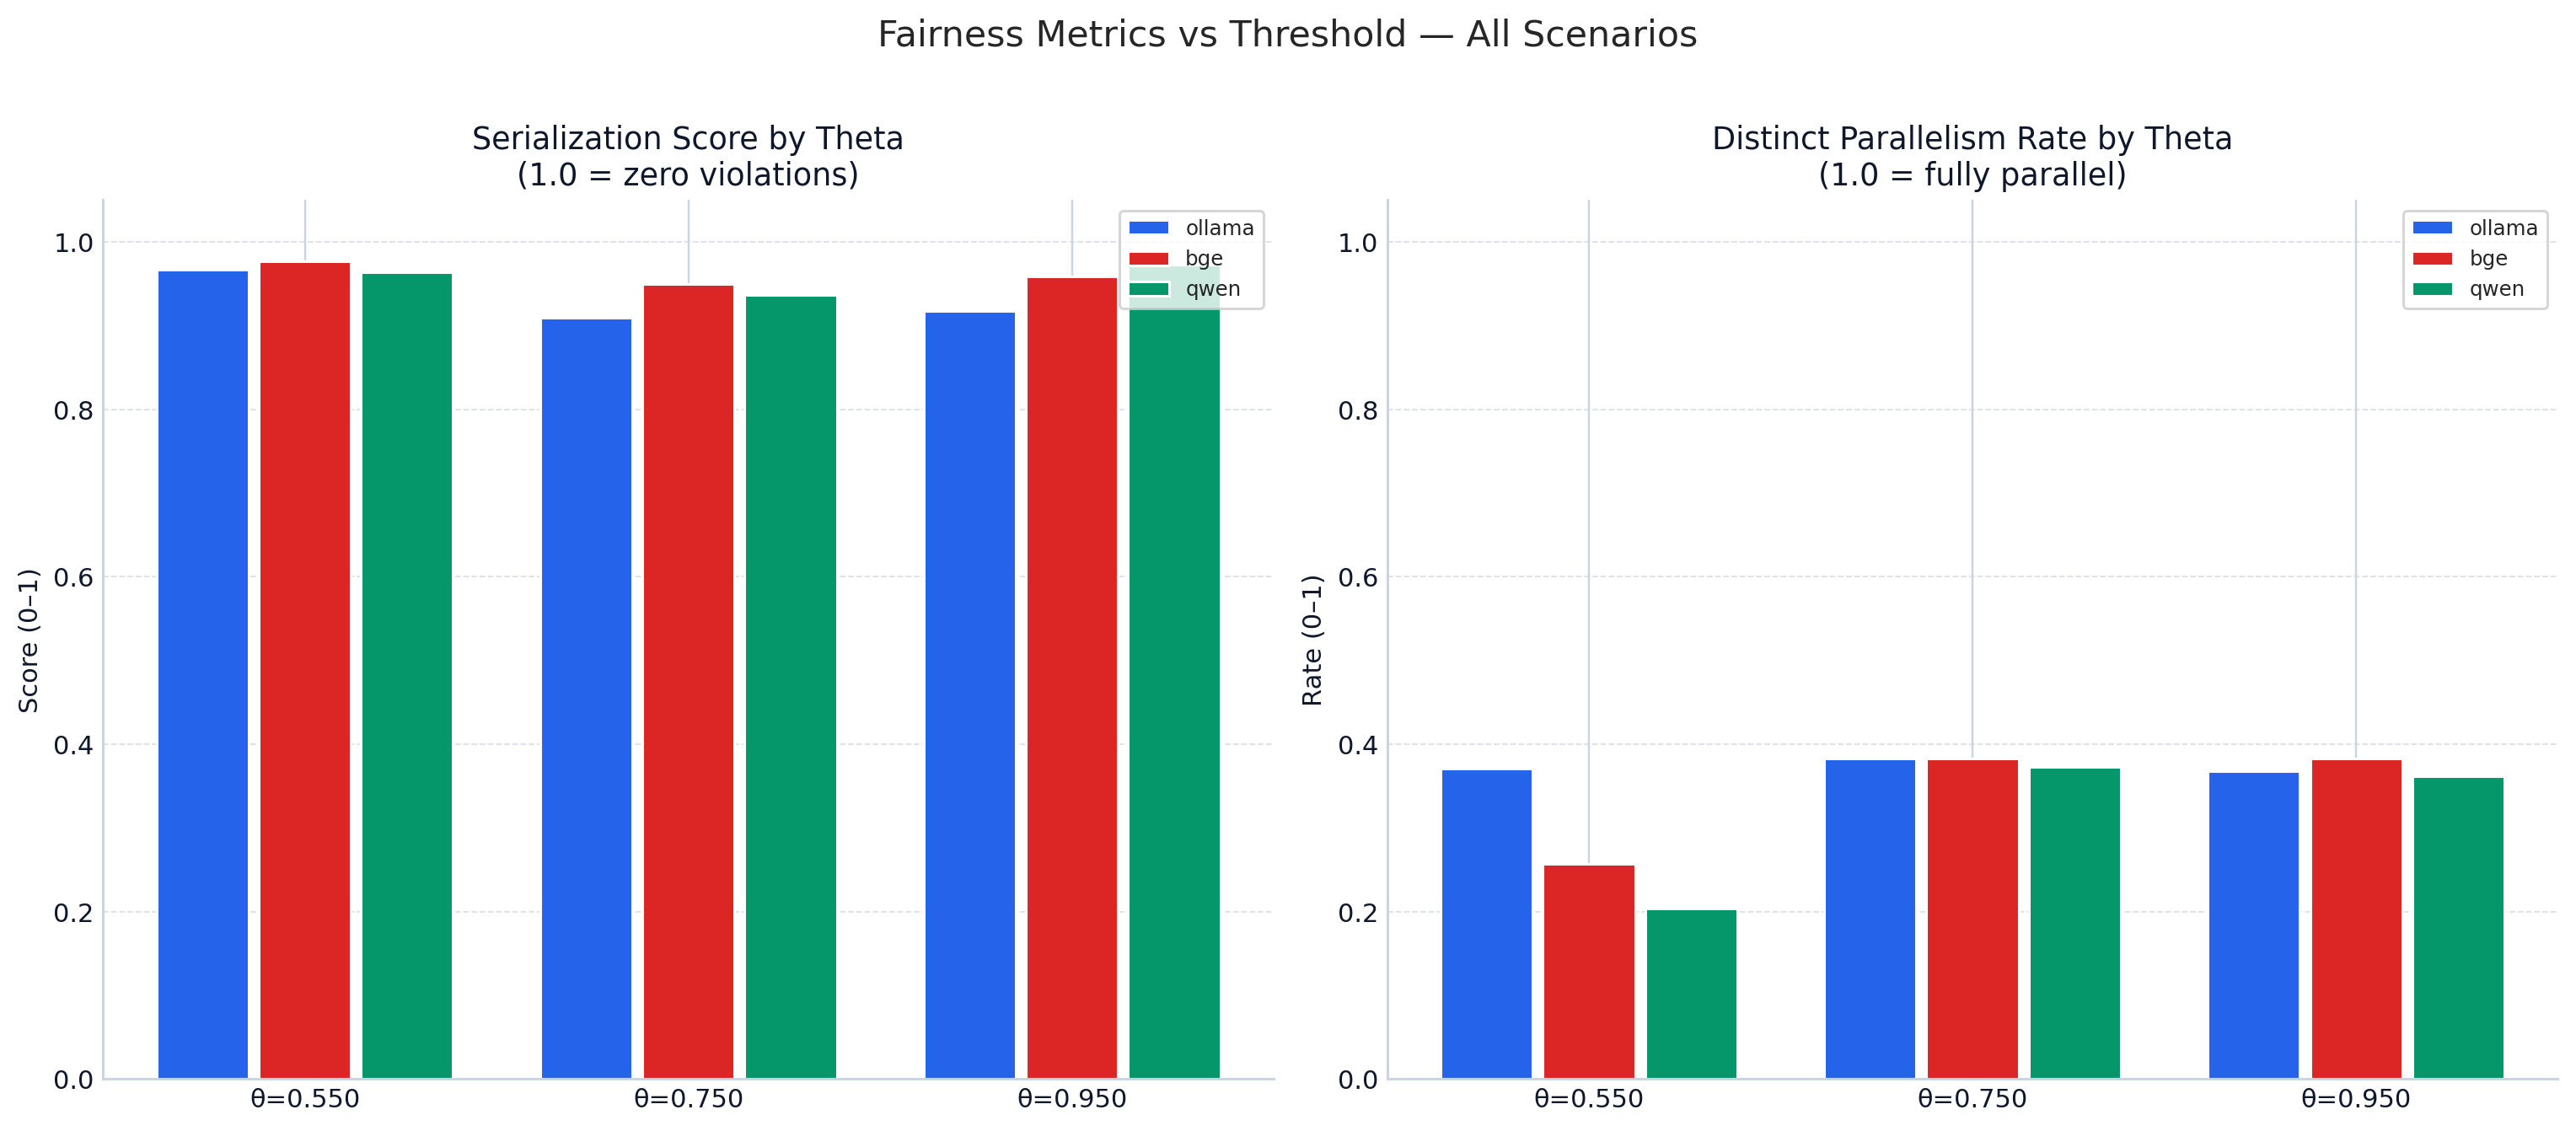
\includegraphics[width=\textwidth,height=4.8cm,keepaspectratio]{scripts/plots/matrix/matrix_02_fairness_by_theta.png}
    \caption{Wait fairness vs.\ $\theta$}
    \label{fig:fairness}
  \end{subfigure}
  \hfill
  \begin{subfigure}[b]{0.48\columnwidth}
    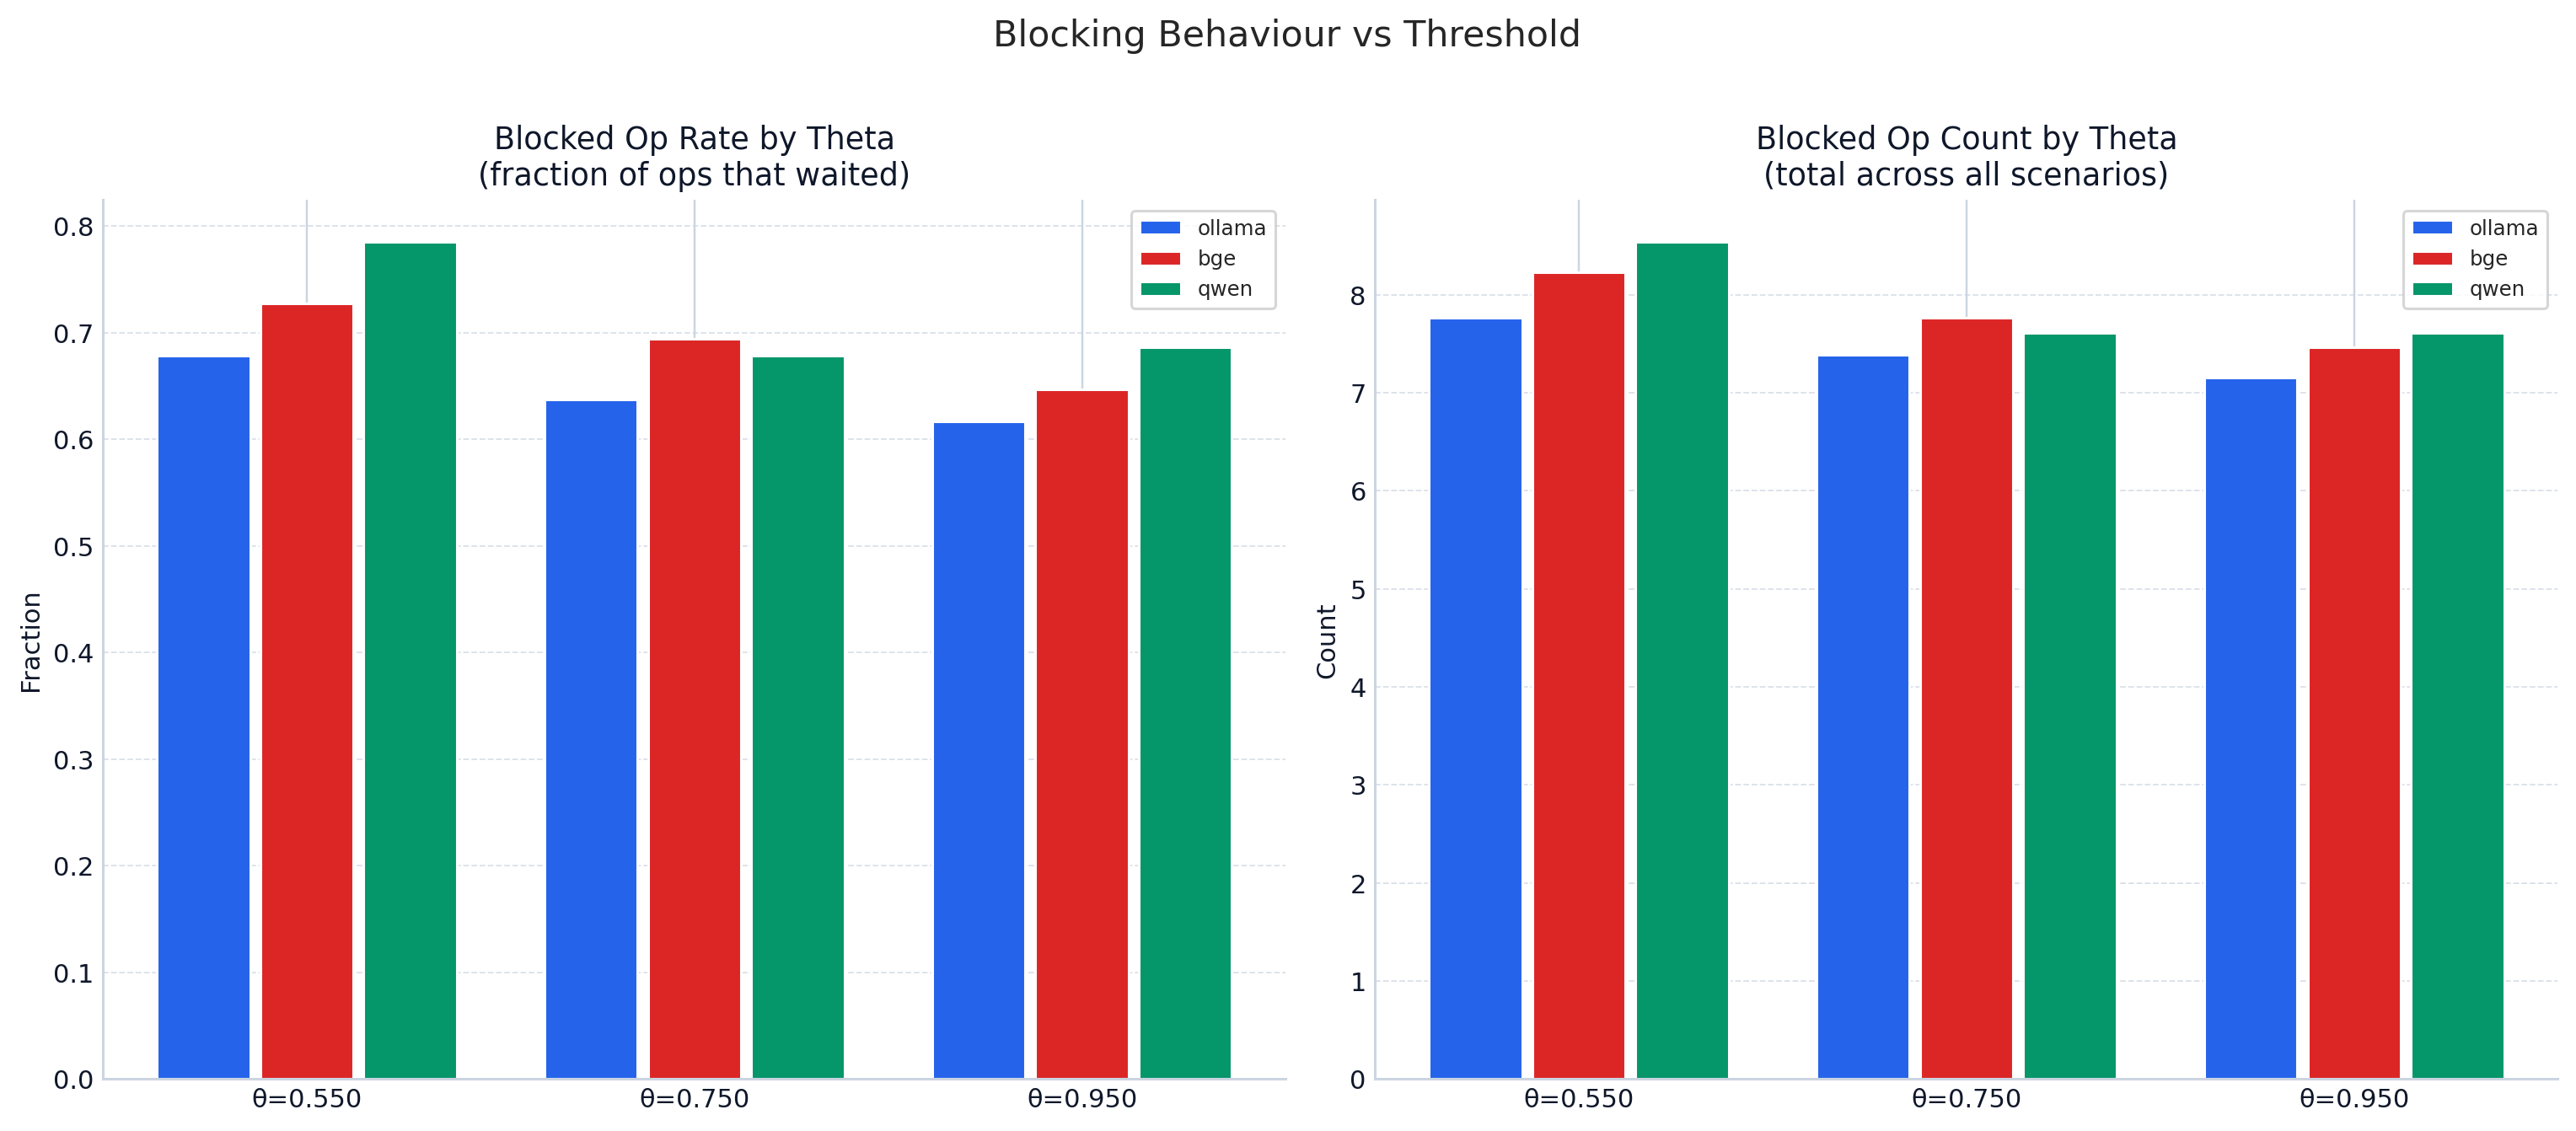
\includegraphics[width=\textwidth,height=4.8cm,keepaspectratio]{scripts/plots/matrix/matrix_03_blocked_rate_by_theta.png}
    \caption{Blocked rate vs.\ $\theta$}
    \label{fig:blocked}
  \end{subfigure}
  \caption{Matrix benchmark results across all model-threshold combinations. Fairness
    and blocked rate are model-agnostic at $\theta{=}0.75$; they become model-specific
    at extremes.}
  \label{fig:matrix}
\end{figure}

Figure~\ref{fig:matrix} shows wait fairness and blocked rate across the full matrix.
At $\theta{=}0.75$, the FIFO rebalancer produces near-uniform fairness across all three
models: the per-waiter CV design ensures that no thread waits longer than its queue
position warrants. At $\theta{=}0.55$, \texttt{bge-m3} and \texttt{qwen3} block a large
fraction of cross-domain requests, degrading fairness as the queue fills with operations
that semantically should not conflict.

\subsection{Resource Utilization}

Per-container resource telemetry was collected via Docker stats snapshots at the end of
each benchmark case. The leader node accounts for the majority of CPU load: it runs the
embedding cosine comparison, the Raft proposal path, and the \texttt{Active\-Lock\-Table}
rebalancer on every acquire/release. Follower nodes spike briefly during
\texttt{AppendEntries} log replication but are otherwise quiescent between heartbeats.
Memory consumption across all nodes is dominated by the in-memory Raft log, which grows
proportionally to the number of committed acquire/release operations and is bounded by the
total number of benchmark operations per run.

\subsection{Locust Load Testing}

We ran sustained Locust~\cite{locust} load tests to characterize throughput at steady
state. Two workloads were tested:

\begin{itemize}
  \item \textbf{Read-only}: 46 RPS, median latency 7\,ms, P95 13\,ms.
  \item \textbf{Write workload}: 32 RPS, median latency 10\,ms, P95 68\,ms.
\end{itemize}

The write workload P95 of 68\,ms includes the Raft consensus round-trip (two heartbeat
periods = 150\,ms upper bound), the Qdrant write, and any queue wait. The P95 being well
below the heartbeat-driven upper bound indicates that the cluster processes most requests
within a single AppendEntries cycle.

\subsection{CAP Positioning}

DSCC deliberately prioritizes Consistency over Availability. An \texttt{AcquireGuard}
request to a partitioned minority cluster (fewer than 3 nodes) will timeout rather than
grant a lock that might conflict with a lock held by the majority. This matches the
intended use case: a semantic race condition in shared agent memory is more harmful than
a temporary unavailability during a network partition.

%% =====================================================================
\section{Limitations and Future Work}
\label{sec:limitations}

\textbf{Sequential vote collection.} Leader election issues \texttt{RequestVote} RPCs
sequentially, giving $O(N \times \text{rpc\_timeout})$ election time in the worst case.
A parallel implementation using \texttt{std::async} or co-routines would reduce this to
$O(\text{rpc\_timeout})$.

\textbf{No pre-vote.} A node that was partitioned and incremented its term will disrupt
the cluster on reconnect by triggering an unnecessary election. The pre-vote extension
to Raft~\cite{raft} would address this; our implementation does not include it.

\textbf{gRPC exponential backoff.} A single dropped packet can push a gRPC channel into
its backoff window, silencing heartbeats and triggering false elections. Channel-level
keepalive tuning or application-level retry budgets would mitigate this.

\textbf{No lock TTL or lease.} A lock held by a crashed agent will remain in the
\texttt{ActiveLockTable} indefinitely, blocking all subsequent conflicting requests.
Lease-based expiry with periodic heartbeating from the agent would allow automatic
cleanup.

\textbf{In-memory Raft log.} The current implementation does not persist the log to disk
or implement log compaction via snapshots. A node that restarts loses its log state and
must rejoin as a fresh follower, potentially requiring log replay from the leader.

\textbf{No lock ownership enforcement.} Any caller can release any lock by agent ID.
A token-based or challenge-response ownership check would prevent accidental or malicious
releases.

\textbf{Future: semantic lock federation.} In large-scale deployments with many agents
and diverse semantic domains, a single lock table may become a bottleneck. Partitioning
the lock space by embedding cluster — effectively sharding semantic regions across
multiple DSCC clusters — is an open design question.

%% =====================================================================
\section{Conclusion}
\label{sec:conclusion}

We presented DSCC, a distributed lock manager that extends the classical conflict
predicate from key identity to semantic similarity. The core contribution — the
\textbf{ActiveLockTable} with per-lock FIFO queues and per-waiter condition variables —
eliminates thundering-herd contention while preserving FIFO fairness through a cascading
grant rebalancer. A two-phase admission protocol integrates the lock table with a
five-node Raft cluster, and a ghost-lock prevention mechanism ensures that failed
consensus proposals leave no permanent residue in the lock table.

Our embedding model evaluation demonstrates that the choice of model is an architectural
commitment, not an implementation detail: the same conflict threshold can produce zero
violations or six violations depending on which model maps the payload into vector space.
We recommend \texttt{qwen3-embedding:0.6b} at $\theta{=}0.75$ as the calibrated
operating point, the only tested combination to achieve a perfect Paraphrase Gauntlet
serialization score.

DSCC demonstrates that semantic concurrency control is tractable for multi-agent shared
memory systems at the throughputs and latencies expected in LLM agent pipelines, opening
a path toward memory-safe multi-agent architectures that do not rely on application-level
deduplication or post-hoc conflict resolution.

%% =====================================================================
\section*{Author Contributions}

\textbf{Ashwattha Phatak}: Designed and implemented the \texttt{Acquire\-Guard} critical
path, the \texttt{Active\-Lock\-Table} (including the per-waiter CV design, the
rebalancer, pending lock semantics, and the cascading grant effect), the gRPC proto
definitions, and the embedding model evaluation study. Designed and ran the
cosine-similarity conflict predicate calibration experiments.

\textbf{Ayush Gala}: Designed and implemented the Raft consensus layer
(\texttt{RaftNode}), the leader election and log replication subsystems, the benchmark
harness (all 13 cases), node lifecycle management, the Locust load testing framework,
and the leader-aware \texttt{dscc-proxy}.

%% =====================================================================
\begin{acks}
This work was completed as the final project for CSC\,724: Advanced Topics in Distributed
Systems at North Carolina State University, Spring 2026. We thank the course instructors
for their feedback and for providing the computational resources used in benchmarking.
\end{acks}

%% =====================================================================
\bibliographystyle{ACM-Reference-Format}
\begin{thebibliography}{99}

\bibitem{chubby}
M.~Burrows.
\newblock The {Chubby} lock service for loosely-coupled distributed systems.
\newblock In {\em Proceedings of the 7th USENIX Symposium on Operating Systems
  Design and Implementation (OSDI)}, pages 335--350, 2006.

\bibitem{zookeeper}
P.~Hunt, M.~Konar, F.~P. Junqueira, and B.~Reed.
\newblock {ZooKeeper}: Wait-free coordination for internet-scale systems.
\newblock In {\em Proceedings of the 2010 USENIX Annual Technical Conference
  (USENIX ATC)}, 2010.

\bibitem{redlock}
S.~Sanfilippo.
\newblock Distributed locks with {Redis}.
\newblock \url{https://redis.io/docs/manual/patterns/distributed-locks/}, 2016.

\bibitem{raft}
D.~Ongaro and J.~Ousterhout.
\newblock In search of an understandable consensus algorithm.
\newblock In {\em Proceedings of the 2014 USENIX Annual Technical Conference
  (USENIX ATC)}, pages 305--320, 2014.

\bibitem{gray1976granularity}
J.~N. Gray, R.~A. Lorie, G.~R. Putzolu, and I.~L. Traiger.
\newblock Granularity of locks and degrees of consistency in a shared data base.
\newblock In {\em Modelling in Data Base Management Systems}, pages 365--394.
  North-Holland, 1976.

\bibitem{kung1981optimistic}
H.~T. Kung and J.~T. Robinson.
\newblock On optimistic methods for concurrency control.
\newblock {\em ACM Transactions on Database Systems}, 6(2):213--226, 1981.

\bibitem{bernstein1983multiversion}
P.~A. Bernstein and N.~Goodman.
\newblock Multiversion concurrency control --- theory and algorithms.
\newblock {\em ACM Transactions on Database Systems}, 8(4):465--483, 1983.

\bibitem{garcia-molina1983}
H.~Garcia-Molina and K.~Salem.
\newblock Semantic concurrency control.
\newblock In {\em Proceedings of the 1983 ACM SIGMOD International Conference
  on Management of Data}, pages 220--224, 1983.

\bibitem{qdrant}
{Qdrant Team}.
\newblock {Qdrant}: Vector similarity search engine and vector database.
\newblock \url{https://qdrant.tech}, 2023.

\bibitem{faiss}
J.~Johnson, M.~Douze, and H.~J\'{e}gou.
\newblock Billion-scale similarity search with {GPUs}.
\newblock {\em IEEE Transactions on Big Data}, 7(3):535--547, 2021.

\bibitem{hnswlib}
Y.~A. Malkov and D.~A. Yashunin.
\newblock Efficient and robust approximate nearest neighbor search using
  {Hierarchical Navigable Small World} graphs.
\newblock {\em IEEE Transactions on Pattern Analysis and Machine Intelligence},
  42(4):824--836, 2020.

\bibitem{langgraph}
{LangChain, Inc.}
\newblock {LangGraph}: Building stateful, multi-actor applications with {LLMs}.
\newblock \url{https://github.com/langchain-ai/langgraph}, 2024.

\bibitem{autogen}
Q.~Wu, G.~Bansal, J.~Zhang, Y.~Wu, B.~Li, E.~Zhu, L.~Jiang, X.~Zhang,
  S.~Zhang, J.~Liu, A.~Awadallah, R.~White, D.~Burger, and C.~Wang.
\newblock {AutoGen}: Enabling next-gen {LLM} applications via multi-agent
  conversation.
\newblock {\em arXiv preprint arXiv:2308.08155}, 2023.

\bibitem{park2023generative}
J.~S. Park, J.~C. O'Brien, C.~J. Cai, M.~R. Morris, P.~Liang, and
  M.~S. Bernstein.
\newblock Generative agents: Interactive simulacra of human behavior.
\newblock In {\em Proceedings of the 36th Annual ACM Symposium on User Interface
  Software and Technology (UIST)}, 2023.

\bibitem{yao2023react}
S.~Yao, J.~Zhao, D.~Yu, N.~Du, I.~Shafran, K.~Narasimhan, and Y.~Cao.
\newblock {ReAct}: Synergizing reasoning and acting in language models.
\newblock In {\em Proceedings of the 11th International Conference on Learning
  Representations (ICLR)}, 2023.

\bibitem{locust}
{Locust Contributors}.
\newblock Locust: An open source load testing tool.
\newblock \url{https://locust.io}, 2024.

\end{thebibliography}

\end{document}
